% Template LaTeX untuk Ujian Kualifikasi
% Program Studi Doktor Informatika
% Universitas Telkom

% Document Class
\documentclass[12pt,a4paper]{report}

% Packages
\usepackage[utf8]{inputenc}
\usepackage[T1]{fontenc}
\usepackage{mathptmx} % Times New Roman
\usepackage{courier}  % Courier for monospace
\usepackage{helvet}   % Helvetica for sans-serif
\usepackage{amsmath}
% \usepackage[english,indonesian]{babel}
\usepackage{geometry}
\usepackage{setspace}
\usepackage{titlesec}
\usepackage{graphicx}
\usepackage{float}
\usepackage{hyperref}
\usepackage{booktabs}
\usepackage{array}
\usepackage[format=hang,font=footnotesize,labelfont=bf]{caption}
\usepackage{enumitem}
\usepackage{parskip}
\usepackage{fancyhdr}
\usepackage{tocloft}
\usepackage{tabularx}
\usepackage{longtable}
\usepackage{ragged2e}
\usepackage[normalem]{ulem} % Added ulem package

% Page Setup
\geometry{
    top=3cm,
    bottom=3cm,
    left=4cm,
    right=3cm
}

% Title Formatting
\titleformat{\chapter}[display]
  {\normalfont\fontsize{16}{19}\bfseries\centering}
  {\chaptertitlename\ \thechapter}
  {0.5em}
  {}
\titlespacing*{\chapter}{0pt}{-20pt}{20pt}
\renewcommand{\chaptername}{BAB}

\titleformat{\section}
    {\normalfont\fontsize{14}{16}\bfseries}{\thesection}{1em}{}
    
\titleformat{\subsection}
    {\normalfont\fontsize{12}{14}\bfseries}{\thesubsection}{1em}{}

\titleformat{\subsubsection}
    {\normalfont\fontsize{12}{14}\normalfont}{\thesubsubsection}{1em}{}

% Spacing
\onehalfspacing

% Header/Footer
\pagestyle{fancy}
\fancyhf{}
\fancyfoot[C]{\thepage}
\renewcommand{\headrulewidth}{0pt}

% Hyperref setup
\hypersetup{
    colorlinks=true,
    linkcolor=black,
    citecolor=black,
    filecolor=black,
    urlcolor=black,
}

% Table of Contents customization
\renewcommand{\contentsname}{DAFTAR ISI}
\renewcommand{\cfttoctitlefont}{\hfill\fontsize{16}{19}\selectfont\bfseries}
\renewcommand{\cftaftertoctitle}{\hfill}
\renewcommand{\cftchappresnum}{BAB }
\setlength{\cftchapnumwidth}{4em}

% List of Tables customization
\renewcommand{\listtablename}{DAFTAR TABEL}
\renewcommand{\cftlottitlefont}{\hfill\fontsize{16}{19}\selectfont\bfseries}
\renewcommand{\cftafterlottitle}{\hfill}

% List of Figures customization
\renewcommand{\listfigurename}{DAFTAR GAMBAR}
\renewcommand{\cftloftitlefont}{\hfill\fontsize{16}{19}\selectfont\bfseries}
\renewcommand{\cftafterloftitle}{\hfill}

% List of Equations setup
\newcommand{\listequationsname}{DAFTAR RUMUS}
\newlistof{myequations}{equ}{\listequationsname}
\newcommand{\myequations}[1]{%
\addcontentsline{equ}{myequations}{\protect\numberline{\theequation}#1}\par}
\renewcommand{\cftequtitlefont}{\hfill\fontsize{16}{19}\selectfont\bfseries}
\renewcommand{\cftafterequtitle}{\hfill}
\setlength{\cftmyequationsindent}{0pt}

% Redefine \listofequations to use the custom list
\newcommand{\listofequations}{\listofmyequations}

% Subsection numbering format (Standard LaTeX numbering is preferred)

% Custom Commands for Metadata
\makeatletter
\newcommand{\myTitle}[1]{\def\@myTitle{#1}}
\newcommand{\myAuthorOne}[2]{\def\@myNameOne{#1}\def\@myNIMOne{#2}}
\newcommand{\myAuthorTwo}[2]{\def\@myNameTwo{#1}\def\@myNIMTwo{#2}}
\newcommand{\myYear}[1]{\def\@myYear{#1}}

% Redefine title page
% Initialize default values
\def\@myTitle{Judul Penelitian}
\def\@myNameOne{Nama Mahasiswa 1}
\def\@myNIMOne{NIM 1}
\def\@myNameTwo{Nama Mahasiswa 2}
\def\@myNIMTwo{NIM 2}
\def\@myYear{Tahun}

\renewcommand{\maketitle}{
    \begin{titlepage}
        \centering
        \vspace*{0.5cm}
        
        % Judul Penelitian
        {\fontsize{14}{16}\selectfont\bfseries
        \@myTitle\par}
        
        \vspace{1.5cm}
        
        % Jenis Laporan
        {\fontsize{12}{14}\selectfont
        \textbf{LAPORAN PROYEK II}\par}
        \vspace{0.5cm}
        {\fontsize{12}{14}\selectfont
        Diajukan untuk Memenuhi Kelulusan Matakuliah Proyek 2 pada Program Studi DIV Teknik Informatika\par}
        
        \vspace{1.5cm}
        
        % Logo
        \IfFileExists{logo.png}{
            \includegraphics[width=0.4\textwidth]{logo.png}
        }{
            {\fontsize{16}{19}\bfseries Logo\par}
        }

        \vspace{1.5cm}
        
        % Penulis
        {\fontsize{12}{14}\selectfont
        \textbf{DISUSUN OLEH :}\par}
        \vspace{0.5cm}
        
        \begin{tabular}{ll}
            \textbf{\@myNIMOne} & \textbf{\@myNameOne} \\
            \textbf{\@myNIMTwo} & \textbf{\@myNameTwo}
        \end{tabular}\par
        
        \vfill
        
        % Program Studi dan Informasi
        {\fontsize{14}{16}\selectfont\bfseries
        PROGRAM STUDI DIV TEKNIK INFORMATIKA\par
        SEKOLAH VOKASI\par
        UNIVERSITAS LOGISTIK DAN BISNIS INTERNASIONAL\par
        BANDUNG\par
        \@myYear\par}
        
    \end{titlepage}
    \newpage
}
\makeatother

% Set Metadata
\myTitle{IMPLEMENTASI SISTEM INFORMASI PEMINJAMAN SARANA DAN PRASARANA KAMPUS BERBASIS WEB MENGGUNAKAN CRUD RDBMS}
\myAuthorOne{MUHAMMAD ARIF RIVALDI}{714240008}
\myAuthorTwo{RADITYA RIZKI RAHARJA}{714240041}
\myYear{2026}

% Bibliography Style
\usepackage[
    backend=bibtex,
    style=authoryear,
    sorting=nyt,
    maxbibnames=99,
    dashed=false,
    url=false,
    doi=true,
]{biblatex}
\urlstyle{same}
\addbibresource{references.bib}
\addbibresource{ref_proyek2.bib}

\begin{document}

% Title Page
\maketitle

% Start Roman Numbering
\pagenumbering{roman}

% Placeholder for Front Matter (can be populated later)
% % LEMBAR PENGESAHAN

\clearpage
\newgeometry{left=1.5cm, right=1.5cm, top=3cm, bottom=3cm}

% Offset footer agar nomor halaman tetap di tengah halaman asli
\fancyhfoffset[L]{1.25cm}
\fancyhfoffset[R]{-1.25cm}

\phantomsection
\addcontentsline{toc}{chapter}{LEMBAR PENGESAHAN}

\vfill

\begin{center}
    {\fontsize{14}{16}\selectfont\bfseries LEMBAR PENGESAHAN}
\end{center}

\vspace{0.8cm}

\begin{center}
    {\bfseries\fontsize{12}{14}\selectfont
    IMPLEMENTASI SISTEM INFORMASI PEMINJAMAN SARANA DAN\\
    PRASARANA KAMPUS BERBASIS WEB MENGGUNAKAN CRUD RDBMS}
\end{center}

\vspace{0.8cm}

\begin{center}
    Diajukan untuk Memenuhi Kelulusan Matakuliah Proyek 2 \\
    Program Studi D-IV Teknik Informatika
    
    \vspace{1cm}
    Disusun Oleh:
    
    \vspace{0.3cm}
    \begin{tabular}{lc}
        Muhammad Arif Rivaldi & 714240008 \\
        Raditya Rizki Raharja & 714240041
    \end{tabular}
\end{center}

\vspace{1.5cm}

% --- Bagian Tanda Tangan Dosen (Simetris & Sejajar) ---
\noindent
\begin{minipage}[t]{0.48\textwidth}
    \begin{center}
        Dosen Pembimbing
        \vspace{2.5cm} 
        
        Rolly Maulana Awangga, S.T., MT., CAIP, SFPC\\
        NIK. 118.72.251
    \end{center}
\end{minipage}%
\hfill%
\begin{minipage}[t]{0.48\textwidth}
    \begin{center}
        Koordinator Proyek 2
        \vspace{2.5cm} 
        
        Rd. Nuraini Siti Fathonah, S.S., M.Hum., SFPC\\
        NIK : 117.86.219
    \end{center}
\end{minipage}

\vspace{2cm}

% --- Bagian Menyetujui ---
\begin{center}
    Menyetujui\\
    Ketua Program Studi DIV Teknik Informatika
    
    \vspace{2.5cm}
    
    Roni Andarsyah, S.T., M.Kom., SFPC\\
    \underline{NIK. 115.88.193}
\end{center}

\vfill

% Reset footer offset
\fancyhfoffset[L]{0cm}
\fancyhfoffset[R]{0cm}
\restoregeometry

% \chapter*{KATA PENGANTAR}
\addcontentsline{toc}{chapter}{KATA PENGANTAR}

\vspace{1cm}
% Isi kata pengantar akan ditambahkan di sini.
Puji syukur kehadirat Allah SWT atas segala rahmat-Nya sehingga laporan ini dapat tersusun hingga selesai.



% DAFTAR ISI
\phantomsection
\addcontentsline{toc}{chapter}{DAFTAR ISI}
\tableofcontents
\clearpage

% DAFTAR GAMBAR
\phantomsection
\addcontentsline{toc}{chapter}{DAFTAR GAMBAR}
\listoffigures
\clearpage

% DAFTAR TABEL
\phantomsection
\addcontentsline{toc}{chapter}{DAFTAR TABEL}
\listoftables
\clearpage

\chapter*{ABSTRAK}
\addcontentsline{toc}{chapter}{ABSTRAK}

\vspace{1cm}
% Isi abstrak akan ditambahkan di sini.

\clearpage

% Start Arabic Numbering for Chapters
\pagenumbering{arabic}
\setcounter{page}{1}

% Placeholder for Chapters
\chapter{PENDAHULUAN}
\hyphenpenalty=10000
\exhyphenpenalty=10000
\sloppy

\section{Deskripsi Aplikasi}
Transformasi digital telah menjadi kebutuhan strategis bagi institusi pendidikan tinggi dalam meningkatkan efisiensi operasional dan kualitas layanan akademik \parencite{Ramdany2024}. Konsep \textit{smart campus} yang memanfaatkan teknologi informasi seperti \textit{cloud computing}, \textit{big data}, dan infrastruktur jaringan terintegrasi, menawarkan peluang untuk mengoptimalkan berbagai aspek pengelolaan kampus \parencite{Nachandiya2018}. Sarana dan prasarana merupakan komponen pendukung utama kegiatan akademik dan non-akademik, sehingga pengelolaannya perlu dilakukan secara terencana dan terdokumentasi. Namun, pada banyak institusi pendidikan, pengelolaan dan peminjaman fasilitas masih dilakukan secara manual atau menggunakan media pencatatan terpisah seperti \textit{Microsoft Excel}, yang berpotensi menimbulkan kesulitan pencarian data, keterlambatan laporan, serta rendahnya efisiensi kerja pengelola \parencite{PutriNabella2025}.

Perkembangan teknologi informasi mendorong penerapan sistem informasi berbasis web sebagai solusi atas permasalahan tersebut. Sistem berbasis web memungkinkan pengelolaan data secara terpusat, mudah diakses, serta mendukung proses pengajuan, pencatatan, dan pelaporan peminjaman fasilitas secara lebih efektif dan terstruktur \parencite{Purwati2022}. Penyajian informasi peminjaman secara \textit{real-time} dapat meminimalkan kesalahan informasi dan bentrok jadwal penggunaan fasilitas kampus \parencite{Herlambang2020}. Integrasi data dan otomatisasi proses dalam sistem informasi juga terbukti memberikan manfaat signifikan terhadap efisiensi operasional dan peningkatan kualitas layanan \parencite{Ramdany2024}.

Berdasarkan kondisi tersebut, dikembangkan Sistem Informasi Peminjaman Sarana dan Prasarana Kampus Berbasis Web menggunakan CRUD RDBMS sebagai solusi terintegrasi dalam pengelolaan peminjaman fasilitas. Sistem ini dirancang untuk mendukung proses pengajuan, persetujuan, serta pendokumentasian peminjaman secara efektif, transparan, dan akuntabel.

\newpage

\section{Rumusan Masalah}
Berdasarkan latar belakang yang telah diuraikan sebelumnya, maka permasalahan dalam Proyek II ini dapat dirumuskan dalam bentuk pertanyaan sebagai berikut:
\begin{enumerate}
    \item Bagaimana merancang sistem informasi berbasis web yang mampu mengelola proses peminjaman sarana dan prasarana kampus secara efektif, terintegrasi, dan terkomputerisasi?
    \item Bagaimana menyediakan mekanisme pengajuan dan pemantauan status peminjaman sarana dan prasarana kampus yang mudah diakses oleh mahasiswa secara real-time?
    \item Bagaimana sistem informasi dapat meminimalkan terjadinya bentrok jadwal peminjaman serta mendukung pengelolaan data peminjaman yang terdokumentasi dengan baik untuk keperluan pelaporan dan evaluasi?
\end{enumerate}

\section{Tujuan}
Berdasarkan rumusan masalah yang telah diuraikan sebelumnya, maka tujuan dari pelaksanaan Proyek II ini adalah sebagai berikut:
\begin{enumerate}
    \item Untuk merancang dan membangun sistem informasi peminjaman sarana dan prasarana kampus berbasis web yang terintegrasi guna mendukung proses pengelolaan fasilitas kampus secara efektif dan terstruktur.
    \item Untuk menyediakan mekanisme pengajuan serta pemantauan status peminjaman sarana dan prasarana kampus yang mudah diakses oleh mahasiswa secara real-time.
    \item Untuk meminimalkan terjadinya bentrok jadwal peminjaman melalui fitur validasi jadwal serta menyediakan pengelolaan data peminjaman yang terdokumentasi dengan baik guna mendukung keperluan pelaporan dan evaluasi.
\end{enumerate}

\newpage

\section{Lingkup Dokumentasi}
Ruang lingkup dokumentasi dalam laporan ini meliputi:
\begin{enumerate}
    \item Perancangan dan implementasi sistem peminjaman sarana dan prasarana kampus yang mencakup proses pengajuan, persetujuan, dan pencatatan kehadiran peminjam.
    \item Analisis kebutuhan fungsional dan non-fungsional sistem yang mendukung pengelolaan peminjaman secara terintegrasi.
    \item Pengelolaan data inventaris sarana dan prasarana yang dibatasi pada operasi tambah, ubah (edit), dan hapus data, tanpa mencakup proses pengadaan atau manajemen stok lanjutan.
\end{enumerate}

\chapter{LANDASAN TEORI}
\hyphenpenalty=10000
\exhyphenpenalty=10000
\sloppy

\section{Tinjauan Pustaka}
Penelitian mengenai pengembangan sistem informasi manajemen aset dan peminjaman telah banyak dilakukan untuk mengatasi permasalahan operasional di institusi pendidikan maupun pemerintahan. \textcite{Purwati2022} mengembangkan sistem informasi peminjaman peralatan jaringan dan multimedia menggunakan metode \textit{Waterfall}. Sistem ini dibangun berbasis \textit{website} dengan bahasa pemrograman PHP dan basis data MySQL. Kelebihan penelitian ini adalah keberhasilannya dalam menggantikan pencatatan manual yang rentan hilang, namun penggunaan metode \textit{Waterfall} dinilai kurang fleksibel terhadap perubahan kebutuhan pengguna yang terjadi di tengah proses pengembangan karena sifatnya yang sekuensial.

Dalam konteks manajemen sarana yang lebih luas, \textcite{PutriNabella2025} melakukan penelitian terkait sistem manajemen sarana dan prasarana (Sarpras), IT, serta laboratorium dengan menggunakan metode \textit{Rational Unified Process} (RUP). Sistem ini dikembangkan menggunakan \textit{framework} CodeIgniter 4 dan MySQL untuk memusatkan data aset yang sebelumnya tersebar dalam file Excel. Penelitian ini unggul dalam standarisasi dokumentasi dan integrasi data untuk keperluan audit. Meskipun demikian, pendekatan RUP yang digunakan cenderung berat pada dokumentasi dan kurang adaptif dibandingkan pendekatan \textit{Agile} dalam merespons umpan balik pengguna secara cepat selama fase pengembangan.

Terkait penerapan metodologi yang lebih adaptif, \textcite{Rifky2022} menerapkan kerangka kerja \textit{Scrum} dalam pengembangan sistem informasi pendataan bangunan. Penelitian ini menggunakan PHP dan \textit{framework} CodeIgniter dengan arsitektur MVC. Hasil studi menunjukkan bahwa \textit{Scrum} efektif diterapkan pada proyek dengan batasan waktu yang ketat dan mampu mengakomodasi perubahan fitur yang dinamis melalui mekanisme \textit{sprint}. Sejalan dengan itu, \textcite{Velasquez-Jimenez2025} juga mengimplementasikan perangkat lunak manajemen inventaris menggunakan metodologi \textit{Scrum} yang diuji menggunakan \textit{System Usability Scale} (SUS), yang membuktikan bahwa pendekatan iteratif meningkatkan kepuasan pengguna dan akurasi data inventaris.

\clearpage
Selain aspek metodologi, aspek kinerja teknis \textit{backend} juga menjadi fokus dalam pengembangan sistem modern. \textcite{Pratama2025} melakukan analisis komparatif kinerja RESTful API menggunakan bahasa pemrograman Go, PHP, dan JavaScript dengan metode Raw SQL dan ORM. Temuan penelitian ini menunjukkan bahwa penggunaan bahasa Go dengan metode Raw SQL memberikan kinerja tertinggi dalam menangani beban permintaan dan efisiensi memori dibandingkan PHP. Hal ini mengindikasikan bahwa untuk sistem yang membutuhkan pemrosesan data cepat dan \textit{real-time}, pemilihan teknologi \textit{backend} sangat krusial, aspek yang sering kali kurang diperhatikan dalam penelitian sistem informasi peminjaman sebelumnya yang mayoritas masih berbasis PHP konvensional.

Berdasarkan paparan penelitian terdahulu, mayoritas pengembangan sistem informasi peminjaman sarana prasarana masih didominasi oleh penggunaan metode tradisional seperti \textit{Waterfall} atau RUP, yang memiliki keterbatasan dalam fleksibilitas adaptasi kebutuhan. Di sisi lain, meskipun metode \textit{Scrum} telah diterapkan pada sistem pendataan bangunan dan inventaris, penerapannya secara spesifik pada sistem peminjaman sarana kampus yang mengintegrasikan konsep \textit{CRUD} RDBMS yang optimal, pemrosesan \textit{real-time}, serta prinsip \textit{green computing} masih belum banyak dieksplorasi. Penelitian ini hadir untuk mengisi celah tersebut (\textit{research gap}) dengan mengusulkan pengembangan sistem informasi peminjaman sarana dan prasarana berbasis web menggunakan metode \textit{Scrum} untuk menjamin fleksibilitas pengembangan, serta mengadopsi teknologi yang mendukung efisiensi sumber daya dan kinerja tinggi guna mendukung operasional kampus yang berkelanjutan.

\section{Sistem Informasi dan Manajemen Sarana Prasarana}
Sistem informasi merupakan sistem terintegrasi yang mengombinasikan manusia, perangkat keras, perangkat lunak, jaringan, dan basis data untuk mengolah serta menyajikan informasi guna mendukung operasional dan pengambilan keputusan dalam organisasi \parencite{Herlambang2020}. Dalam konteks perguruan tinggi, sistem informasi menjadi instrumen utama transformasi digital untuk menggantikan proses pengelolaan sarana dan prasarana yang masih manual atau semi-digital, sehingga informasi dapat disajikan secara cepat, akurat, dan konsisten \parencite{Purwati2022}.

Sarana dan prasarana kampus merupakan aset pendukung penting bagi kegiatan akademik dan non-akademik, sehingga pengelolaannya memerlukan manajemen yang sistematis. Proses peminjaman sarana dan prasarana umumnya mencakup tahapan pengajuan, verifikasi ketersediaan, persetujuan, penjadwalan, hingga pengembalian aset. Dalam konteks operasional kampus, proses peminjaman tersebut juga melibatkan peran petugas keamanan sebagai pihak yang memastikan kesesuaian antara jadwal peminjaman pada sistem dengan penggunaan sarana secara aktual di lapangan. Implementasi proses tersebut dalam sistem informasi berbasis web memungkinkan integrasi data inventaris dan transaksi peminjaman secara terpusat serta mendukung pemantauan ketersediaan fasilitas secara \textit{real-time} \parencite{PutriNabella2025}.

Pengelolaan sarana dan prasarana yang masih dilakukan secara manual atau menggunakan \textit{spreadsheet} terpisah berpotensi menimbulkan berbagai permasalahan, seperti redundansi data, keterlambatan pelaporan, dan risiko bentrok jadwal peminjaman akibat keterbatasan informasi ketersediaan fasilitas \parencite{Herlambang2020}. Oleh karena itu, diperlukan sistem informasi peminjaman sarana dan prasarana kampus yang terintegrasi sebagai landasan perancangan sistem pada penelitian ini.

\section{Metodologi \textit{Scrum}}
Pengembangan sistem informasi peminjaman sarana dan prasarana kampus menuntut metode yang mampu beradaptasi terhadap perubahan kebutuhan pengguna selama proses transformasi dari sistem manual ke digital. Berdasarkan penelitian terdahulu, kerangka kerja \textit{Scrum} terbukti efektif dalam pengembangan sistem dengan kebutuhan dinamis dan batasan waktu yang ketat karena mendukung pengembangan bertahap serta validasi berulang pada setiap iterasi \parencite{Rifky2022, Velasquez-Jimenez2025}. Oleh karena itu, \textit{Scrum} dinilai relevan untuk digunakan dalam penelitian ini guna meminimalkan risiko ketidaksesuaian fungsi sistem dengan kebutuhan operasional pengguna.

\textit{Scrum} didefinisikan sebagai kerangka kerja \textit{Agile} yang bersifat iteratif dan inkremental untuk menghasilkan solusi adaptif terhadap permasalahan kompleks melalui transparansi, inspeksi, dan adaptasi \parencite{Schwaber2012}. Dalam penerapannya, \textit{Scrum} melibatkan peran utama \textit{Product Owner}, \textit{Scrum Master}, dan \textit{Development Team}, serta didukung oleh artefak \textit{Product Backlog}, \textit{Sprint Backlog}, dan \textit{Increment} yang dikelola melalui serangkaian event seperti \textit{Sprint Planning}, \textit{Daily Scrum}, \textit{Sprint Review}, dan \textit{Sprint Retrospective} \parencite{permana2015scrum, Nugraha2021}. Karakteristik tersebut menjadikan \textit{Scrum} sebagai landasan metodologis yang sesuai untuk pengembangan sistem peminjaman sarana kampus secara modular dan adaptif, yang pada penelitian ini akan diimplementasikan melalui mekanisme \textit{sprint} pada tahap perancangan dan pengembangan sistem di Bab 3.

\section{Basis Data Relasional dan Konsep \textit{CRUD}}
Sistem peminjaman sarana dan prasarana kampus melibatkan pengelolaan data yang kompleks, mencakup data pengguna, inventaris aset, serta jadwal pemakaian yang bersifat dinamis. Pengelolaan data yang masih dilakukan secara manual atau menggunakan \textit{spreadsheet} terpisah sering menimbulkan permasalahan berupa data yang tidak terintegrasi, kesulitan penelusuran riwayat transaksi, serta keterlambatan penyusunan laporan. Kondisi serupa juga ditemukan pada berbagai institusi pendidikan, di mana keterbatasan sistem pencatatan konvensional berdampak pada rendahnya efisiensi dan akurasi pengelolaan sarana dan prasarana \parencite{PutriNabella2025}.

Pendekatan yang umum digunakan untuk mengatasi permasalahan tersebut adalah penerapan \textit{Relational Database Management System} (RDBMS), yaitu sistem manajemen basis data yang mengorganisasikan data ke dalam tabel-tabel yang saling berelasi melalui kunci utama (\textit{primary key}) dan kunci asing (\textit{foreign key}). Struktur relasional memungkinkan integrasi data secara terpusat, menjaga konsistensi informasi, serta mendukung akses data lintas unit kerja secara \textit{real-time}, sebagaimana diterapkan pada pengembangan sistem manajemen inventaris dan peminjaman di lingkungan pendidikan \parencite{Velasquez-Jimenez2025, Ramdany2024}. Interaksi antara aplikasi dan basis data dalam sistem informasi dilakukan melalui mekanisme \textit{CRUD} (\textit{Create, Read, Update, Delete}), yang merepresentasikan siklus hidup data mulai dari pencatatan aset, pemrosesan peminjaman, hingga pembaruan dan penghapusan data yang tidak lagi relevan \parencite{Purwati2022}.

Untuk menjaga kinerja dan kualitas basis data, diperlukan penerapan teknik normalisasi basis data guna meminimalkan redundansi dan mencegah terjadinya anomali data. Struktur basis data yang ternormalisasi memungkinkan setiap atribut disimpan secara tepat sesuai ketergantungannya, sehingga integritas data tetap terjaga dan efisiensi penyimpanan meningkat. Integrasi antara RDBMS, operasi \textit{CRUD} yang efisien, serta struktur data yang ternormalisasi menjadi landasan teoretis utama dalam perancangan arsitektur data pada penelitian ini, yang implementasi teknisnya akan dibahas lebih lanjut pada Bab 3, sejalan dengan kebutuhan sistem peminjaman yang andal dan berkinerja baik \parencite{Pratama2025}.

\section{Teknologi Sistem Informasi Berbasis Web dengan Prinsip \textit{Green Computing}}
Pengembangan sistem informasi peminjaman sarana dan prasarana kampus memerlukan platform yang mampu mendukung interaksi \textit{multi-user} secara terpusat dengan akses informasi ketersediaan aset secara \textit{real-time} guna meminimalkan bentrok jadwal dan kesalahan pencatatan. Sistem juga harus mengakomodasi akses lintas peran (\textit{role-based access}), mulai dari mahasiswa hingga administrator, untuk menjamin keamanan dan keteraturan alur kerja. Oleh karena itu, teknologi berbasis web dipilih karena mampu mengintegrasikan seluruh proses peminjaman ke dalam satu sistem terpusat yang meningkatkan akurasi data dan efisiensi pelaporan dibandingkan metode manual atau penggunaan \textit{spreadsheet} terpisah \parencite{Herlambang2020, PutriNabella2025, Velasquez-Jimenez2025}.

Secara konseptual, aplikasi web beroperasi menggunakan arsitektur \textit{client–server} yang memungkinkan pemisahan antara antarmuka pengguna dan pemrosesan data di sisi server melalui protokol HTTP. Arsitektur ini menawarkan keunggulan berupa aksesibilitas tinggi, kemudahan integrasi dengan sistem administratif kampus, serta skalabilitas yang baik dalam menangani peningkatan jumlah pengguna \parencite{Purwati2022, Ramdany2024}. Kinerja sistem web sangat bergantung pada komponen \textit{backend} dan pengelolaan basis data dalam menangani logika bisnis serta operasi \textit{CRUD}, di mana efisiensi pemrosesan dan pemilihan metode pengelolaan data yang tepat berperan penting dalam menjaga stabilitas dan waktu respons sistem, terutama pada beban akses yang tinggi \parencite{Pratama2025}.

Sejalan dengan tuntutan keberlanjutan global, pengembangan sistem informasi modern juga harus mengadopsi prinsip efisiensi sumber daya atau \textit{Green Computing}. \textit{Green Computing} atau \textit{Green IT} mencakup praktik perancangan, penggunaan, dan pembuangan sistem komputer dengan dampak lingkungan seminimal mungkin, baik melalui efisiensi energi maupun pengurangan limbah \parencite{Murugesan2012}. Implementasi nyata konsep ini dalam sistem peminjaman adalah penerapan \textit{paperless office}, yang mendigitalkan formulir dan laporan untuk mengurangi konsumsi kertas dan emisi karbon secara signifikan \parencite{Kim2021}. Lebih jauh lagi, prinsip ini juga diterapkan pada level desain perangkat lunak, di mana algoritma dan kode program dioptimalkan untuk meminimalkan beban kerja prosesor dan memori, sehingga mengurangi konsumsi energi operasional server \parencite{Pratama2025}.

\section{Pengujian Perangkat Lunak}
Pengujian perangkat lunak merupakan tahapan fundamental dalam siklus pengembangan sistem untuk menjamin kebenaran, kelengkapan, dan kualitas produk akhir. \textcite{taley2020comprehensive} menjelaskan bahwa pengujian tidak hanya bertujuan untuk menemukan kesalahan (\textit{bugs}), tetapi juga memverifikasi dan memvalidasi bahwa perangkat lunak telah memenuhi persyaratan teknis serta kebutuhan pengguna sebelum dirilis. Dalam konteks pengembangan sistem informasi manajemen, pengujian yang sistematis diperlukan untuk memastikan bahwa alur kerja yang kompleks, seperti proses peminjaman dan validasi data, dapat berjalan tanpa hambatan dan risiko kegagalan fungsi dapat diminimalisir \parencite{Suwirmayanti2020}.

Salah satu metode utama yang digunakan untuk memvalidasi fungsionalitas sistem adalah \textit{Black Box Testing}. Metode ini berfokus pada pengujian spesifikasi fungsional perangkat lunak tanpa perlu mengetahui struktur kode internal atau logika pemrograman di dalamnya \parencite{Suwirmayanti2020}. Pengujian ini dilakukan dengan memberikan serangkaian input pada antarmuka sistem dan mengevaluasi kesesuaian output yang dihasilkan dengan hasil yang diharapkan \parencite{PutriNabella2025}. Pendekatan ini sangat relevan untuk sistem peminjaman sarana kampus guna memastikan bahwa fitur-fitur kritikal, seperti formulir pengajuan, validasi stok aset, autentikasi pengguna, serta skenario validasi penggunaan sarana di lapangan oleh pihak terkait, berfungsi dengan benar sesuai skenario penggunaan (\textit{use case}) yang telah dirancang \parencite{Purwati2022}.

Selain validasi fungsional, evaluasi kualitas teknis pada sisi \textit{backend} dilakukan menggunakan pengukuran \textit{Code Coverage}. \textit{Code Coverage} adalah metrik yang digunakan untuk mengukur seberapa banyak baris kode program yang telah dieksekusi selama proses pengujian otomatis (\textit{unit testing}). Dalam pengembangan \textit{backend} menggunakan bahasa pemrograman Go (Golang), pengujian dan pengukuran coverage didukung secara bawaan oleh pustaka \texttt{testing} dan perintah \texttt{go test} \parencite{kommadi2019learn}. Penggunaan alat ini memungkinkan pengembang untuk mengidentifikasi bagian logika program yang belum teruji (\textit{uncovered code}) dan memastikan bahwa fungsi-fungsi krusial, seperti operasi \textit{CRUD} dan logika bisnis, memiliki tingkat keterujian yang tinggi sebelum integrasi sistem dilakukan.

Kombinasi antara \textit{Black Box Testing} untuk validasi eksternal dan \textit{Code Coverage} untuk validasi internal membentuk strategi pengujian yang komprehensif. Landasan teori ini menjadi dasar bagi pelaksanaan pengujian sistem yang hasil dan analisisnya akan dipaparkan secara mendetail pada Bab 4 Implementasi dan Pengujian, guna membuktikan bahwa sistem informasi peminjaman sarana dan prasarana yang dibangun telah memenuhi standar kualitas yang ditetapkan.

\chapter{METODOLOGI PENELITIAN}
\hyphenpenalty=10000
\exhyphenpenalty=10000
\sloppy

\section{Jenis dan Metode Penelitian}
Pemilihan metode dan pendekatan penelitian pada pengembangan Sistem Informasi Peminjaman Sarana dan Prasarana Kampus disesuaikan dengan karakteristik permasalahan yang dihadapi serta kebutuhan pengguna sistem. Permasalahan pengelolaan peminjaman fasilitas kampus yang masih dilakukan secara manual dan semi-digital menuntut adanya solusi sistem informasi yang terstruktur, adaptif, dan mampu mendukung proses operasional secara efektif. Oleh karena itu, metode dan pendekatan penelitian yang digunakan diarahkan untuk menghasilkan sistem yang tidak hanya memenuhi kebutuhan fungsional pengguna, tetapi juga mampu diimplementasikan secara optimal dalam lingkungan operasional kampus.

\subsection{Jenis Penelitian}
Penelitian ini merupakan penelitian terapan (\textit{applied research}) yang berfokus pada pengembangan sistem informasi untuk mendukung proses peminjaman sarana dan prasarana kampus. Penelitian terapan dipilih karena tujuan utama penelitian ini bukan hanya menghasilkan kajian teoritis, tetapi juga menghasilkan produk perangkat lunak yang dapat digunakan secara langsung untuk menyelesaikan permasalahan nyata yang terjadi di lingkungan kampus.

Pendekatan yang digunakan dalam penelitian ini adalah rekayasa perangkat lunak, di mana proses penelitian meliputi analisis kebutuhan, perancangan sistem, pengembangan aplikasi, serta pengujian fungsional sistem.

\subsection{Metode Penelitian}
Metode penelitian yang digunakan adalah Scrum, yaitu salah satu metode pengembangan perangkat lunak berbasis Agile yang bersifat iteratif dan inkremental. Pemilihan metode Scrum didasarkan pada karakteristik permasalahan yang ditemukan dari hasil observasi dan wawancara dengan staf Sarana dan Prasarana kampus, antara lain:
\newpage
\begin{enumerate}
    \item Kebutuhan sistem yang dinamis dan dapat berubah seiring proses pengembangan.
    \item Keterlibatan banyak pemangku kepentingan (Mahasiswa/UKM, Staf Sarpras, dan Security).
    \item Perlunya evaluasi berkala terhadap sistem yang dikembangkan agar sesuai dengan kebutuhan pengguna.
\end{enumerate}
Metode Scrum memungkinkan pengembangan sistem dilakukan secara bertahap melalui beberapa \textit{sprint}, sehingga setiap tahapan pengembangan dapat dievaluasi dan disempurnakan berdasarkan umpan balik pengguna \parencite{Nugraha2021}.

\subsection{Objek dan Subjek Penelitian}
\subsubsection{Objek Penelitian}
Objek penelitian dalam penelitian ini adalah Sistem Informasi Peminjaman Sarana dan Prasarana Kampus ULBI, yang mencakup proses pengelolaan jadwal ruangan, pengajuan peminjaman, verifikasi peminjaman, validasi kehadiran, serta pembuatan laporan peminjaman secara terintegrasi. Sistem ini dirancang untuk menggantikan proses manual dan semi-digital yang sebelumnya digunakan, sehingga diharapkan dapat meningkatkan efisiensi, akurasi data, serta transparansi proses peminjaman.

\subsubsection{Subjek Penelitian}
Subjek penelitian adalah pihak-pihak yang terlibat langsung dalam penggunaan sistem, yaitu:
\begin{enumerate}
    \item Mahasiswa/UKM, sebagai pihak pemohon peminjaman sarana dan prasarana.
    \item Staf Sarana dan Prasarana, sebagai pihak pengelola dan pemberi persetujuan peminjaman.
    \item Petugas Keamanan (Security), sebagai pihak yang melakukan validasi kehadiran dan izin kegiatan di lapangan.
\end{enumerate}
Penentuan subjek penelitian ini mengacu pada hasil analisis kebutuhan dan \textit{Use Case Diagram} yang menggambarkan interaksi aktor dengan sistem.

\subsection{Teknik Pengumpulan Data}
\subsubsection{Observasi}
Teknik observasi dilakukan dengan mengamati secara langsung proses peminjaman sarana dan prasarana yang berjalan di lingkungan kampus. Observasi difokuskan pada proses pencatatan jadwal, pengajuan peminjaman, serta mekanisme verifikasi kegiatan yang masih dilakukan secara manual atau semi-digital. Hasil observasi digunakan sebagai dasar untuk mengidentifikasi permasalahan operasional yang terjadi pada sistem lama.

\subsubsection{Wawancara}
Wawancara dilakukan dengan staf Sarana dan Prasarana sebagai pihak yang bertanggung jawab dalam pengelolaan peminjaman fasilitas kampus. Wawancara bertujuan untuk:
\begin{enumerate}
    \item Menggali kebutuhan sistem yang diharapkan.
    \item Mengidentifikasi kendala dalam proses peminjaman yang sedang berjalan.
    \item Menentukan fitur utama yang harus tersedia dalam sistem.
\end{enumerate}
Hasil wawancara ini kemudian dirangkum dalam dokumen spesifikasi kebutuhan perangkat lunak (SKPL).

\subsubsection{Studi Pustaka}
Pengelolaan sarana dan prasarana di institusi pendidikan memerlukan sistem informasi yang terintegrasi untuk mengatasi permasalahan pencatatan manual, keterlambatan informasi, serta kesulitan dalam penyusunan laporan. Penelitian sebelumnya menunjukkan bahwa sistem informasi manajemen sarana dan prasarana mampu meningkatkan efisiensi pengelolaan fasilitas, mempercepat proses administrasi, serta mempermudah monitoring penggunaan aset di lingkungan pendidikan \parencite{Nabella2025}.

Dalam pengembangan sistem informasi berbasis web, metode Agile khususnya Scrum banyak digunakan karena mampu menangani kebutuhan sistem yang bersifat dinamis dan melibatkan banyak pemangku kepentingan. Scrum menerapkan pengembangan secara iteratif dan inkremental melalui tahapan \textit{product backlog}, \textit{sprint planning}, \textit{sprint}, \textit{sprint review}, dan \textit{sprint retrospective}, sehingga memungkinkan sistem dikembangkan secara bertahap sesuai kebutuhan pengguna \parencite{Nugraha2021}.

Penerapan Scrum pada sistem informasi sektor publik juga menunjukkan hasil yang efektif. Penelitian mengenai pengembangan Sistem Informasi Pendataan Bangunan (SIPBANG) pada instansi pemerintahan membuktikan bahwa Scrum mampu menghasilkan sistem yang sesuai dengan kebutuhan pengguna meskipun terdapat keterbatasan waktu dan kompleksitas proses bisnis. Evaluasi hasil sprint menunjukkan bahwa sistem yang dikembangkan dengan Scrum lebih adaptif dan mudah disesuaikan dengan kebutuhan organisasi \parencite{Rifky2022}.

Selain itu, kajian metodologis yang mengombinasikan Scrum dengan model pengembangan lain menunjukkan bahwa Scrum memiliki keunggulan dalam fleksibilitas dan pengelolaan perubahan kebutuhan, khususnya pada pengembangan perangkat lunak berbasis website. Pendekatan Scrum dinilai efektif dalam meningkatkan kualitas produk perangkat lunak karena memungkinkan evaluasi dan perbaikan dilakukan secara berkelanjutan pada setiap iterasi pengembangan \parencite{Tumbade2024}.

Pada tahap pengujian sistem, \textit{Black Box Testing} merupakan teknik pengujian yang umum digunakan untuk memastikan fungsionalitas sistem berjalan sesuai dengan spesifikasi yang telah ditentukan. Pengujian ini berfokus pada kesesuaian antara input dan output sistem tanpa memperhatikan struktur internal kode program. Penelitian terdahulu menunjukkan bahwa \textit{Black Box Testing} efektif digunakan untuk menguji kesiapan sistem sebelum digunakan oleh pengguna akhir, khususnya pada sistem berbasis web \parencite{Putra2020}.

Berdasarkan hasil studi pustaka tersebut, dapat disimpulkan bahwa pengembangan sistem informasi manajemen sarana dan prasarana menggunakan metode Scrum serta pengujian \textit{Black Box Testing} merupakan pendekatan yang relevan dan didukung oleh penelitian sebelumnya. Studi pustaka ini menjadi landasan teoritis dalam perancangan dan pengembangan Sistem Informasi Peminjaman Sarana dan Prasarana Kampus pada penelitian ini.

\subsection{Tahapan Metode Penelitian Menggunakan Scrum}
Metode penelitian yang digunakan dalam pengembangan Sistem Informasi Peminjaman Sarana dan Prasarana Kampus adalah Scrum, yang diterapkan secara iteratif dan inkremental. Tahapan Scrum dalam penelitian ini disusun berdasarkan diagram metodologi Scrum yang telah dirancang, sehingga setiap tahapan memiliki luaran yang jelas dan dapat dibuktikan pada tahap hasil penelitian (BAB IV).

\newpage
Berdasarkan diagram metodologi Scrum yang digunakan dalam penelitian ini, proses penelitian dan pengembangan sistem dilakukan secara iteratif dan inkremental, dimulai dari tahap perencanaan produk hingga evaluasi berkelanjutan melalui beberapa siklus sprint.

\begin{figure}[htbp]
    \centering
    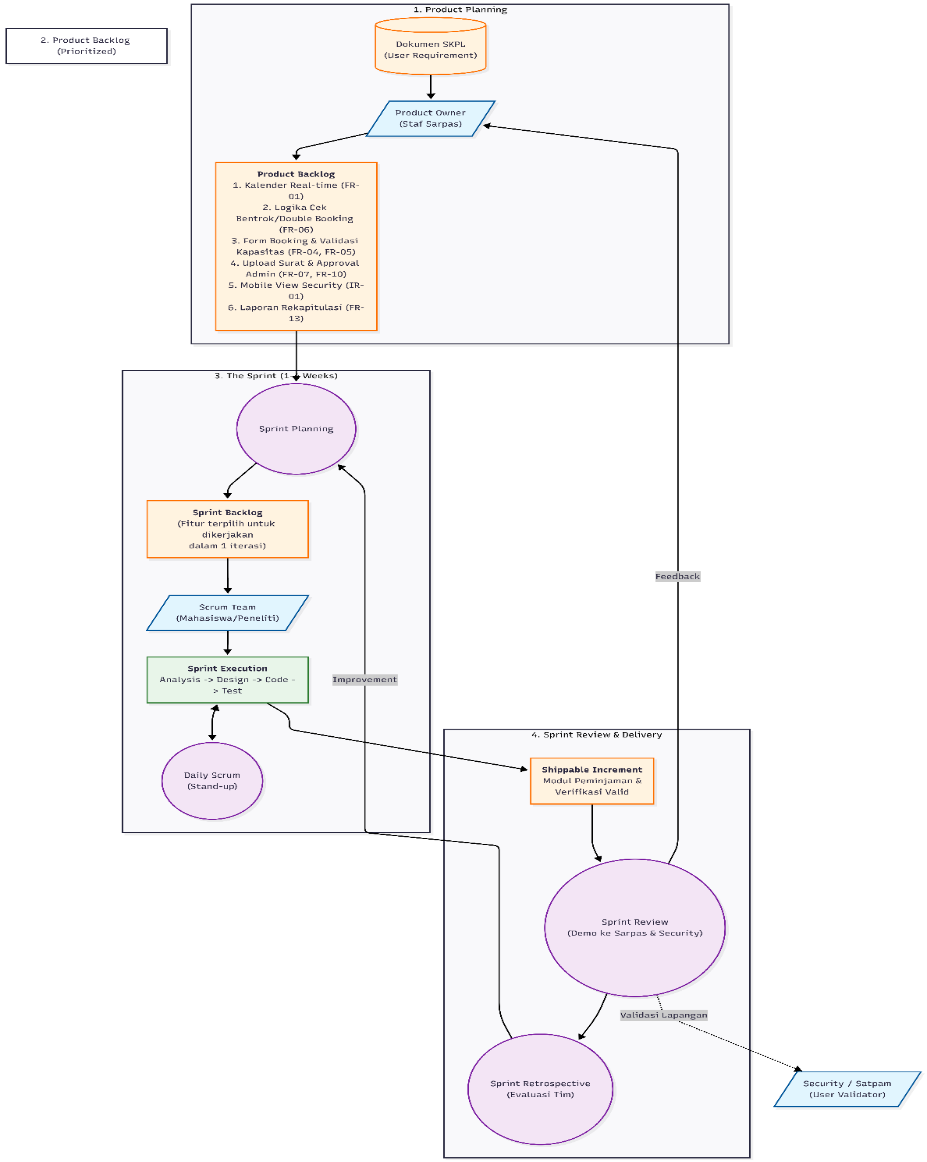
\includegraphics[width=0.8\textwidth]{gambar/media/image2.png}
    \caption{Alur Metode Scrum}
    \label{fig:alur_scrum}
\end{figure}

\subsubsection{Product Planning}
Tahap awal dalam metode Scrum adalah \textit{Product Planning}, yang bertujuan untuk mengidentifikasi dan mendefinisikan kebutuhan sistem secara menyeluruh. Pada tahap ini, kebutuhan sistem diperoleh dari Dokumen Spesifikasi Kebutuhan Perangkat Lunak (SKPL) yang disusun berdasarkan hasil observasi dan wawancara dengan staf Sarana dan Prasarana kampus.

\newpage
Dalam \textit{Product Planning}, \textit{Product Owner}, yang diperankan oleh staf Sarpras, berperan dalam memvalidasi kebutuhan pengguna serta memastikan bahwa kebutuhan tersebut sesuai dengan proses bisnis peminjaman sarana dan prasarana kampus. Tahap ini menghasilkan pemahaman awal terhadap ruang lingkup sistem yang akan dikembangkan.

\subsubsection{Product Backlog}
Berdasarkan hasil \textit{Product Planning}, selanjutnya disusun \textit{Product Backlog}, yaitu daftar kebutuhan sistem yang telah diprioritaskan. \textit{Product Backlog} disusun mengacu pada kebutuhan fungsional yang telah didefinisikan dalam dokumen SKPL dan \textit{Use Case Diagram}.

\textit{Product Backlog} pada penelitian ini mencakup fitur utama seperti kalender ketersediaan ruangan secara real-time, pencegahan bentrok jadwal (\textit{double booking}), form peminjaman dan validasi kapasitas, unggah surat digital dan persetujuan admin, tampilan mobile untuk petugas keamanan, serta fitur laporan rekapitulasi peminjaman. \textit{Product Backlog} ini menjadi dasar perencanaan pengembangan sistem pada setiap \textit{sprint}.

\subsubsection{Sprint Planning}
Setelah \textit{Product Backlog} disusun, dilakukan \textit{Sprint Planning} untuk menentukan item \textit{Product Backlog} yang akan dikerjakan dalam satu iterasi pengembangan. \textit{Sprint Planning} dilakukan dengan mempertimbangkan prioritas kebutuhan pengguna dan kemampuan tim pengembang.

Hasil dari \textit{Sprint Planning} adalah \textit{Sprint Backlog}, yaitu daftar fitur terpilih yang akan dikembangkan oleh \textit{Scrum Team} dalam satu \textit{sprint}. Pada penelitian ini, durasi setiap \textit{sprint} ditetapkan selama 1–2 minggu.

\subsubsection{Sprint Execution}
Tahap \textit{Sprint Execution} merupakan tahap pelaksanaan pengembangan sistem oleh \textit{Scrum Team}, yang dalam penelitian ini diperankan oleh mahasiswa/peneliti. Pada tahap ini, pengembangan sistem dilakukan secara bertahap yang meliputi analisis kebutuhan fitur, perancangan sistem, implementasi kode program, serta pengujian fungsional awal.

\newpage
Selama \textit{Sprint Execution} berlangsung, dilakukan \textit{Daily Scrum} (\textit{stand-up meeting}) untuk memantau progres pengembangan, mengidentifikasi kendala yang muncul, serta memastikan pekerjaan berjalan sesuai dengan rencana \textit{sprint} yang telah ditetapkan.

\subsubsection{Sprint Review and Delivery}
Setelah \textit{Sprint Execution} selesai, sistem yang telah dikembangkan menghasilkan \textit{Shippable Increment}, yaitu modul sistem yang telah dapat dijalankan dan diuji. Increment ini kemudian dipresentasikan pada tahap \textit{Sprint Review}, yang melibatkan pihak staf Sarpras dan petugas keamanan (Security).

\textit{Sprint Review} bertujuan untuk memperoleh umpan balik pengguna serta melakukan validasi terhadap kesesuaian sistem dengan kebutuhan operasional di lapangan. Hasil \textit{Sprint Review} menjadi dasar perbaikan atau penyesuaian fitur pada \textit{sprint} berikutnya.

\subsubsection{Sprint Retrospective}
Tahap akhir dalam satu siklus \textit{sprint} adalah \textit{Sprint Retrospective}, yaitu evaluasi internal yang dilakukan oleh \textit{Scrum Team} terhadap proses pengembangan yang telah berlangsung. Evaluasi ini bertujuan untuk mengidentifikasi kekurangan, hambatan, serta peluang perbaikan dalam proses pengembangan sistem. Hasil \textit{Sprint Retrospective} digunakan sebagai dasar perbaikan berkelanjutan (\textit{continuous improvement}) pada \textit{sprint} berikutnya, sehingga kualitas sistem dan proses pengembangan dapat terus ditingkatkan.

\subsection{Teknik Pengujian}
Pengujian sistem pada penelitian ini dilakukan untuk memastikan bahwa Sistem Informasi Peminjaman Sarana dan Prasarana Kampus yang dikembangkan telah berfungsi sesuai dengan kebutuhan pengguna yang telah didefinisikan pada tahap analisis kebutuhan. Pengujian sistem merupakan bagian penting dari proses pengembangan menggunakan metode Scrum, di mana setiap increment sistem yang dihasilkan pada akhir \textit{sprint} harus memenuhi kriteria fungsional yang telah ditetapkan.

\newpage
\subsubsection{Metode Pengujian}
Metode pengujian yang digunakan dalam penelitian ini adalah \textit{Black Box Testing}. \textit{Black Box Testing} merupakan metode pengujian perangkat lunak yang berfokus pada pengujian fungsionalitas sistem tanpa memperhatikan struktur internal atau kode program yang digunakan. Pemilihan metode \textit{Black Box Testing} didasarkan pada pertimbangan bahwa tujuan utama pengujian adalah untuk memastikan bahwa setiap fitur sistem dapat berjalan sesuai dengan kebutuhan pengguna, sebagaimana yang telah dirumuskan dalam dokumen spesifikasi kebutuhan perangkat lunak dan \textit{use case diagram}.

\subsubsection{Ruang Lingkup Pengujian}
Ruang lingkup pengujian sistem mencakup seluruh fitur utama yang dikembangkan pada setiap \textit{sprint}, khususnya fitur-fitur yang berkaitan langsung dengan proses peminjaman sarana dan prasarana kampus. Fitur yang diuji meliputi:
\begin{enumerate}
    \item Fitur login pengguna sesuai dengan hak akses masing-masing aktor.
    \item Fitur tampilan kalender ketersediaan ruangan secara real-time.
    \item Fitur pengajuan peminjaman ruangan dan sarana.
    \item Fitur validasi kapasitas ruangan dan pencegahan \textit{double booking}.
    \item Fitur unggah surat digital dan proses verifikasi oleh admin.
    \item Fitur verifikasi kehadiran oleh petugas keamanan.
    \item Fitur notifikasi status pengajuan dan laporan rekapitulasi peminjaman.
\end{enumerate}
Pengujian dilakukan untuk memastikan bahwa setiap fitur tersebut memberikan keluaran yang sesuai dengan hasil yang diharapkan.

\subsubsection{Skenario dan Prosedur Pengujian}
Pengujian sistem dilakukan dengan menyusun skenario pengujian berdasarkan fungsi-fungsi utama sistem. Setiap skenario pengujian terdiri dari beberapa komponen, yaitu kondisi awal, langkah pengujian, data masukan, hasil yang diharapkan, dan hasil pengujian aktual.

\newpage
Prosedur pengujian dilakukan dengan cara menjalankan sistem sesuai dengan skenario yang telah ditentukan, kemudian membandingkan hasil aktual dengan hasil yang diharapkan. Apabila hasil pengujian sesuai dengan hasil yang diharapkan, maka fitur tersebut dinyatakan berhasil. Sebaliknya, apabila terjadi perbedaan, maka fitur tersebut akan diperbaiki dan diuji kembali pada \textit{sprint} berikutnya.

\subsubsection{Waktu dan Pelaksanaan Pengujian}
Pengujian sistem dilakukan pada akhir setiap \textit{sprint}, setelah tahap \textit{Sprint Execution} selesai. Dengan demikian, setiap increment sistem yang dihasilkan telah melalui proses pengujian sebelum diserahkan pada tahap \textit{Sprint Review}. Pendekatan ini sejalan dengan prinsip Scrum yang menekankan pada pengujian dan evaluasi berkelanjutan, sehingga kesalahan atau kekurangan sistem dapat segera diidentifikasi dan diperbaiki pada \textit{sprint} berikutnya.

\subsubsection{Hasil Pengujian}
Hasil pengujian sistem didokumentasikan dalam bentuk tabel pengujian \textit{Black Box Testing} yang memuat informasi mengenai skenario pengujian, hasil yang diharapkan, hasil aktual, serta status keberhasilan pengujian. Dokumentasi hasil pengujian ini akan disajikan dan dibahas secara rinci pada BAB IV sebagai bukti bahwa sistem yang dikembangkan telah memenuhi kebutuhan fungsional yang ditetapkan.

\section{Analisis Sistem}
Analisis sistem dilakukan untuk mengidentifikasi kebutuhan dan karakteristik Sistem Informasi Peminjaman Sarana dan Prasarana Kampus yang dikembangkan. Analisis ini bertujuan untuk memahami proses bisnis yang berjalan, kebutuhan pengguna, serta fungsi-fungsi yang harus disediakan oleh sistem agar mampu mendukung pengelolaan peminjaman sarana dan prasarana kampus secara efektif, terstruktur, dan terkomputerisasi.

Dalam penelitian ini, teknik analisis data digunakan untuk mengolah dan menafsirkan data yang diperoleh selama proses pengembangan dan pengujian sistem. Analisis data bertujuan untuk menilai kesesuaian antara sistem yang dikembangkan dengan kebutuhan pengguna yang telah ditetapkan pada tahap analisis kebutuhan. Pendekatan analisis data yang digunakan adalah analisis kualitatif, karena data yang dianalisis berupa hasil observasi, wawancara, evaluasi sprint, serta hasil pengujian fungsional sistem.

\subsection{Analisis Kebutuhan Sistem}
Analisis kebutuhan sistem dilakukan dengan mengkaji hasil observasi dan wawancara yang telah dirangkum dalam Dokumen Spesifikasi Kebutuhan Perangkat Lunak (SKPL). Data kebutuhan dianalisis untuk mengidentifikasi permasalahan utama dalam proses peminjaman sarana dan prasarana kampus, seperti pencatatan peminjaman yang belum terintegrasi, kesulitan pemantauan status peminjaman, serta keterbatasan dokumentasi data peminjaman.

Hasil analisis kebutuhan ini digunakan sebagai dasar dalam penyusunan \textit{Product Backlog} serta penentuan prioritas fitur pada setiap \textit{sprint} pengembangan, sehingga sistem yang dikembangkan sesuai dengan kebutuhan pengguna dan proses bisnis yang berjalan.

\subsection{Analisis Fungsional}
Analisis fungsional bertujuan untuk mengidentifikasi fungsi utama yang harus dimiliki oleh Sistem Informasi Peminjaman Sarana dan Prasarana Kampus dalam mendukung proses peminjaman secara terkomputerisasi. Sistem menerapkan konsep CRUD (\textit{Create, Read, Update, Delete}) untuk mengelola data peminjaman dan sarana secara terintegrasi.

Secara fungsional, sistem diawali dengan proses autentikasi pengguna untuk membatasi hak akses. Mahasiswa dapat mengajukan peminjaman sarana dan prasarana, sementara admin bertugas mengelola data sarana, memverifikasi, serta menyetujui atau menolak pengajuan peminjaman. Seluruh data peminjaman disimpan dalam basis data dan statusnya dapat dipantau oleh pengguna.

Berdasarkan analisis tersebut, kebutuhan fungsional sistem meliputi:
\begin{enumerate}
    \item Fitur notifikasi status pengajuan dan laporan rekapitulasi peminjaman.
    \item Autentikasi dan login pengguna berdasarkan hak akses.
    \item Pengajuan peminjaman sarana dan prasarana oleh mahasiswa.
    \item Penampilan informasi ketersediaan dan riwayat peminjaman.
    \item Persetujuan atau penolakan peminjaman oleh sarpras.
    \item Pengelolaan data sarana dan prasarana menggunakan operasi CRUD.
    \item Penyediaan laporan data peminjaman.
\end{enumerate}
Analisis kebutuhan fungsional ini menjadi dasar dalam tahap perancangan sistem yang dibahas pada subbab selanjutnya.

\subsection{Analisis Non-Fungsional}
Analisis non-fungsional dilakukan untuk mengidentifikasi kebutuhan pendukung yang memastikan Sistem Informasi Peminjaman Sarana dan Prasarana Kampus dapat berjalan secara optimal, aman, dan mudah digunakan. Kebutuhan non-fungsional ini tidak berkaitan langsung dengan fungsi utama sistem, tetapi berperan penting dalam menjamin kualitas layanan sistem secara keseluruhan.

Adapun kebutuhan non-fungsional sistem adalah sebagai berikut:
\begin{enumerate}
    \item Keamanan, sistem menerapkan mekanisme autentikasi pengguna untuk membatasi akses sesuai dengan hak akses masing-masing pengguna.
    \item Kinerja (\textit{performance}), sistem mampu memproses data peminjaman dan menampilkan informasi secara responsif.
    \item Ketersediaan (\textit{availability}), sistem dapat diakses melalui \textit{web browser} kapan saja selama terhubung dengan jaringan internet.
    \item \textit{Usability}, antarmuka sistem dirancang agar mudah dipahami dan digunakan oleh pengguna.
    \item Kompatibilitas, sistem dapat dijalankan pada berbagai perangkat dan peramban web.
\end{enumerate}
Dengan adanya kebutuhan non-fungsional ini, sistem diharapkan mampu memberikan layanan peminjaman sarana dan prasarana kampus yang andal, aman, dan nyaman digunakan. Analisis kebutuhan non-fungsional ini selanjutnya menjadi dasar dalam tahap perancangan sistem.

\subsection{Analisis Proses Pengembangan Sistem}
Analisis proses pengembangan sistem dilakukan dengan mengevaluasi pelaksanaan setiap tahapan Scrum yang telah dijalankan. Data yang dianalisis meliputi hasil \textit{Sprint Planning}, \textit{Sprint Execution}, \textit{Sprint Review}, dan \textit{Sprint Retrospective}.

Analisis ini bertujuan untuk menilai efektivitas penerapan metode Scrum dalam pengembangan sistem, serta untuk mengidentifikasi kendala dan perbaikan yang dilakukan selama proses pengembangan berlangsung.

\subsection{Analisis Hasil Pengujian Sistem}
Analisis hasil pengujian sistem dilakukan dengan mengkaji hasil pengujian \textit{Black Box Testing} terhadap fitur-fitur utama sistem. Data pengujian dianalisis dengan membandingkan hasil aktual sistem dengan hasil yang diharapkan pada setiap skenario pengujian.

Fitur yang memenuhi kriteria pengujian dinyatakan berfungsi dengan baik, sedangkan fitur yang belum memenuhi kriteria akan diperbaiki dan diuji kembali pada \textit{sprint} berikutnya.

\section{Perancangan}
Perancangan sistem dilakukan sebagai tahap lanjutan dari hasil analisis kebutuhan fungsional dan non-fungsional yang telah dijelaskan sebelumnya. Tahap ini bertujuan untuk menerjemahkan kebutuhan sistem ke dalam bentuk rancangan teknis yang menggambarkan struktur, alur, dan komponen sistem yang akan dibangun.



\subsection{Usecase Diagram}

\begin{figure}[H]
    \centering
    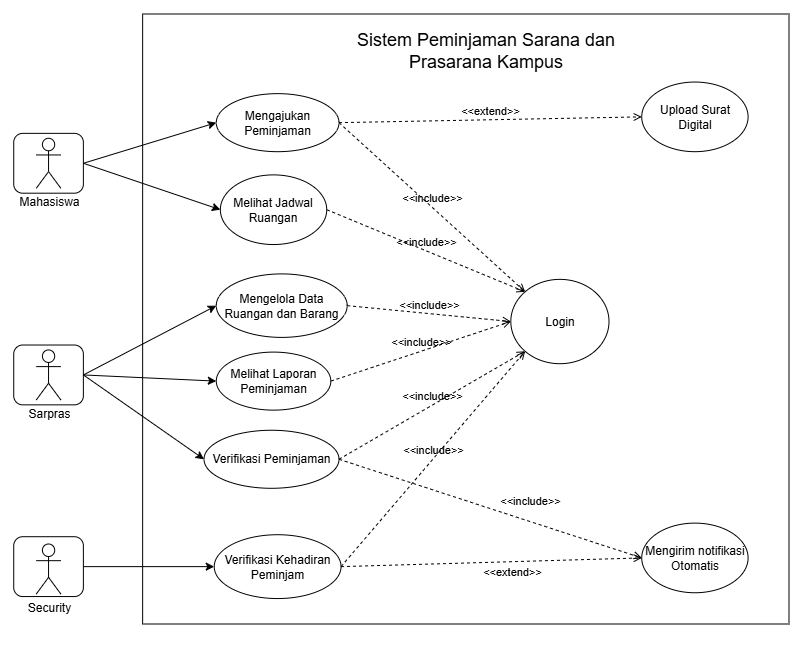
\includegraphics[width=0.8\textwidth]{gambar/media/image3.png}
    \caption{Usecase Diagram}
    \label{fig:usecase_diagram}
\end{figure}

\newpage
Use Case Diagram pada Sistem Informasi Peminjaman Sarana dan Prasarana Kampus menggambarkan interaksi antara aktor dengan sistem berdasarkan hak akses dan peran masing-masing. Penjelasan Use Case Diagram disajikan dalam bentuk tabel aktor dan tabel use case sebagai berikut.

\begin{table}[htbp]
    \centering
    \caption{Usecase Sistem}
    \label{tab:usecase_sistem}
    \begin{tabular}{|c|p{5cm}|p{8.5cm}|}
        \hline
        No. & Usecase & Deskripsi \\
        \hline
        1. & Login & Proses autentikasi pengguna untuk dapat mengakses sistem sesuai dengan hak akses masing-masing. \\
        \hline
        2. & Mengajukan Peminjaman & Proses pengajuan peminjaman sarana dan prasarana kampus dengan mengisi data peminjaman. \\
        \hline
        3. & Upload Surat Digital & Proses unggah dokumen pendukung peminjaman sebagai kelengkapan pengajuan. \\
        \hline
        4. & Melihat Jadwal Ruangan & Proses melihat jadwal penggunaan ruangan untuk menghindari bentrok peminjaman. \\
        \hline
        5. & Mengelola Data Ruangan dan Barang & Proses pengelolaan data sarana dan prasarana kampus menggunakan operasi CRUD. \\
        \hline
        6. & Melihat Laporan Peminjaman & Proses melihat data dan rekap laporan peminjaman sarana dan prasarana kampus. \\
        \hline
        7. & Verifikasi Peminjaman & Proses verifikasi dan persetujuan atau penolakan pengajuan peminjaman yang diajukan mahasiswa. \\
        \hline
        8. & Verifikasi Kehadiran Peminjam & Proses pemeriksaan kehadiran peminjam pada saat penggunaan sarana dan prasarana. \\
        \hline
        9. & Mengirim Notifikasi Otomatis & Proses pengiriman notifikasi secara otomatis sebagai tindak lanjut dari verifikasi kehadiran atau peminjaman. \\
        \hline
    \end{tabular}
\end{table}

\newpage
\begin{table}[htbp]
    \centering
    \caption{Aktor Sistem}
    \label{tab:aktor_sistem}
    \begin{tabular}{|c|l|p{10cm}|}
        \hline
        No. & Aktor & Deskripsi \\
        \hline
        1. & Mahasiswa & Pengguna sistem yang mengajukan peminjaman sarana dan prasarana kampus, melihat jadwal ruangan, serta mengunggah surat digital sebagai dokumen pendukung peminjaman. \\
        \hline
        2. & Sarpras & Pengelola sarana dan prasarana kampus yang bertugas mengelola data ruangan dan barang, melihat laporan peminjaman, serta melakukan verifikasi pengajuan peminjaman. \\
        \hline
        3. & Security & Petugas yang melakukan verifikasi kehadiran peminjam pada saat peminjaman berlangsung dan memicu pengiriman notifikasi otomatis. \\
        \hline
    \end{tabular}
\end{table}

\subsection{Flowchart Diagram}

\subsubsection{Flowchart Pengajuan Peminjaman}
Flowchart Pengajuan peminjaman menggambarkan alur proses pengajuan peminjaman sarana dan prasarana kampus oleh mahasiswa, mulai dari login hingga pengajuan berhasil dikirim ke sistem. Proses ini bertujuan untuk memastikan bahwa pengajuan peminjaman dilakukan secara terstruktur, lengkap, dan sesuai dengan ketentuan yang berlaku.

\begin{figure}[htbp]
    \centering
    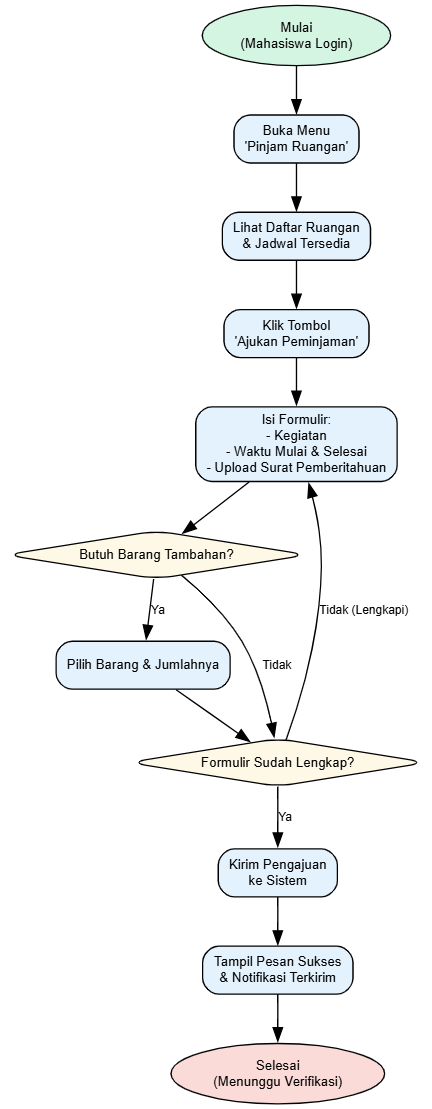
\includegraphics[width=0.6\textwidth]{gambar/media/image4.png}
    \caption{Flowchart Pengajuan Peminjaman}
    \label{fig:flowchart_pengajuan}
\end{figure}

Proses peminjaman dimulai setelah mahasiswa berhasil login dan memilih menu Pinjam Ruangan. Mahasiswa dapat melihat daftar ruangan beserta jadwal ketersediaannya, kemudian mengajukan peminjaman dengan mengisi formulir yang memuat informasi kegiatan, waktu peminjaman, serta mengunggah surat pemberitahuan. Jika diperlukan, mahasiswa dapat menambahkan barang pendukung beserta jumlahnya. Sistem akan memeriksa kelengkapan data, dan apabila telah lengkap pengajuan dikirim dengan status menunggu verifikasi, disertai notifikasi bahwa pengajuan berhasil diajukan.

\newpage
Dengan adanya flowchart peminjaman ini, alur proses pengajuan peminjaman sarana dan prasarana kampus oleh mahasiswa dapat dipahami secara jelas dan terstruktur. Flowchart ini menjadi acuan dalam implementasi fitur peminjaman serta membantu memastikan bahwa setiap pengajuan yang dikirimkan telah melalui proses validasi sebelum dilakukan verifikasi oleh pihak pengelola.


\subsubsection{Flowchart Verifikasi Peminjaman}
Flowchart verifikasi peminjaman menggambarkan alur proses pemeriksaan dan pengambilan keputusan terhadap pengajuan peminjaman sarana dan prasarana kampus yang dilakukan oleh Admin atau Sarpras. Proses ini bertujuan untuk memastikan bahwa pengajuan yang masuk telah memenuhi ketentuan administratif, jadwal penggunaan, serta kelengkapan dokumen pendukung sebelum peminjaman disetujui atau ditolak.

Proses verifikasi peminjaman dimulai ketika Admin atau pihak Sarana dan Prasarana (Sarpras) melakukan login ke dalam sistem informasi peminjaman. Setelah berhasil masuk, Admin diarahkan ke halaman dashboard admin yang menampilkan notifikasi pengajuan peminjaman baru dari mahasiswa sebagai penanda bahwa terdapat permohonan yang perlu ditindaklanjuti.

Selanjutnya, Admin membuka detail pengajuan peminjaman untuk melakukan pemeriksaan secara menyeluruh terhadap data yang diajukan oleh mahasiswa. Pada tahap ini, Admin mengecek kelengkapan dokumen pendukung, seperti surat pemberitahuan atau surat permohonan peminjaman, serta memverifikasi kesesuaian jadwal peminjaman dengan ketersediaan sarana dan prasarana yang diminta. Pemeriksaan ini bertujuan untuk memastikan bahwa pengajuan telah memenuhi ketentuan, prosedur, dan aturan peminjaman yang berlaku di lingkungan kampus.

Setelah seluruh data dan dokumen dinyatakan telah diperiksa, Admin kemudian mengambil keputusan terhadap pengajuan peminjaman tersebut. Apabila pengajuan tidak memenuhi persyaratan atau terjadi ketidaksesuaian jadwal maupun dokumen, Admin dapat menolak pengajuan dengan mengisi alasan penolakan secara jelas dan sistem akan secara otomatis mengubah status peminjaman menjadi \textit{rejected}. Sebaliknya, apabila pengajuan dinyatakan sesuai dan memenuhi seluruh ketentuan, Admin menyetujui permohonan tersebut dan sistem akan mengubah status peminjaman menjadi \textit{approved}.

\begin{figure}[htbp]
    \centering
    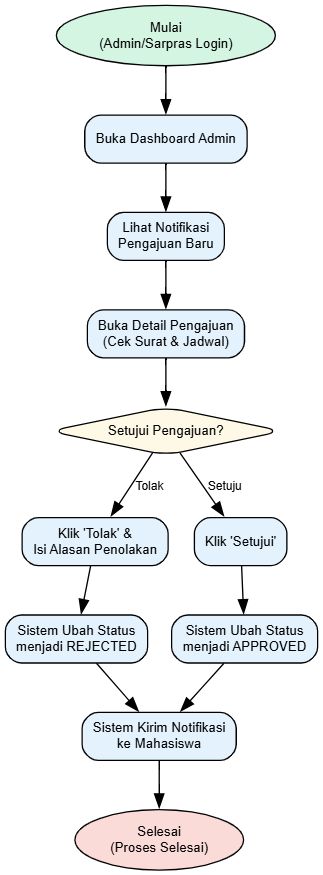
\includegraphics[width=0.6\textwidth]{gambar/media/image5.png}
    \caption{Flowchart Verifikasi Peminjaman}
    \label{fig:flowchart_verifikasi}
\end{figure}

\newpage
Pada tahap akhir, sistem secara otomatis mengirimkan notifikasi kepada mahasiswa mengenai hasil verifikasi peminjaman, baik berupa persetujuan maupun penolakan beserta alasannya. Dengan adanya flowchart verifikasi peminjaman ini, alur pemeriksaan, pengambilan keputusan, dan penyampaian informasi dapat dipahami secara jelas dan sistematis serta menjadi acuan dalam implementasi fitur verifikasi peminjaman agar pengelolaan sarana dan prasarana berjalan lebih efektif dan terstruktur.

\subsubsection{Flowchart Verifikasi Kehadiran Peminjam}
Flowchart verifikasi kehadiran peminjam menggambarkan proses pemeriksaan kehadiran peminjam sarana dan prasarana kampus yang dilakukan oleh petugas security. Proses ini bertujuan untuk memastikan bahwa peminjam yang datang ke lokasi benar-benar sesuai dengan data peminjaman yang telah disetujui sebelumnya oleh pihak Sarpras.

\begin{figure}[htbp]
    \centering
    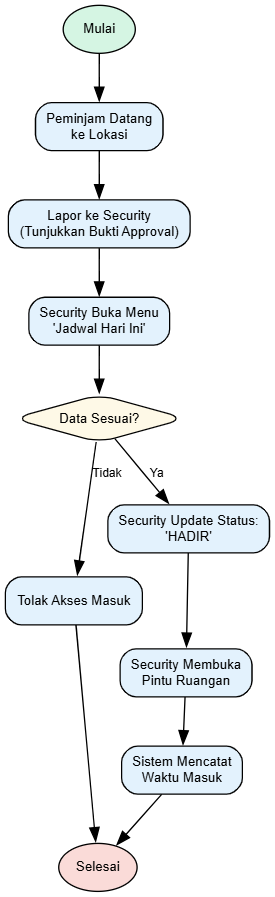
\includegraphics[width=0.4\textwidth]{gambar/media/image6.png}
    \caption{Flowchart Verifikasi Kehadiran Peminjam}
    \label{fig:flowchart_kehadiran}
\end{figure}

Proses verifikasi kehadiran dimulai ketika peminjam datang ke lokasi dan melapor kepada petugas security dengan menunjukkan bukti persetujuan peminjaman. Petugas kemudian membuka menu Jadwal Hari Ini untuk memeriksa data peminjaman yang terjadwal. Sistem menampilkan data peminjaman, lalu petugas melakukan pengecekan kesesuaian identitas peminjam. Jika data tidak sesuai, akses ditolak dan proses dihentikan. Jika sesuai, petugas memperbarui status kehadiran menjadi HADIR, membuka akses ruangan, dan sistem secara otomatis mencatat waktu masuk peminjam. Proses verifikasi kehadiran kemudian dinyatakan selesai.

Flowchart verifikasi kehadiran ini berfungsi sebagai acuan dalam pengawasan penggunaan sarana dan prasarana kampus, sehingga proses peminjaman dapat berlangsung secara tertib, aman, dan terkontrol.

\newpage
\subsection{Sequence Diagram}

\subsubsection{Sequence Diagram Pengajuan Peminjaman}
Sequence diagram ini menggambarkan alur interaksi antara Mahasiswa, Web App, System, Database, dan Email Service dalam proses pengajuan peminjaman ruangan. Proses dimulai ketika mahasiswa melakukan login melalui Web App. Permintaan login divalidasi oleh System dengan melakukan pengecekan data ke Database. Jika data valid, sistem menampilkan dashboard kepada mahasiswa.

\begin{figure}[htbp]
    \centering
    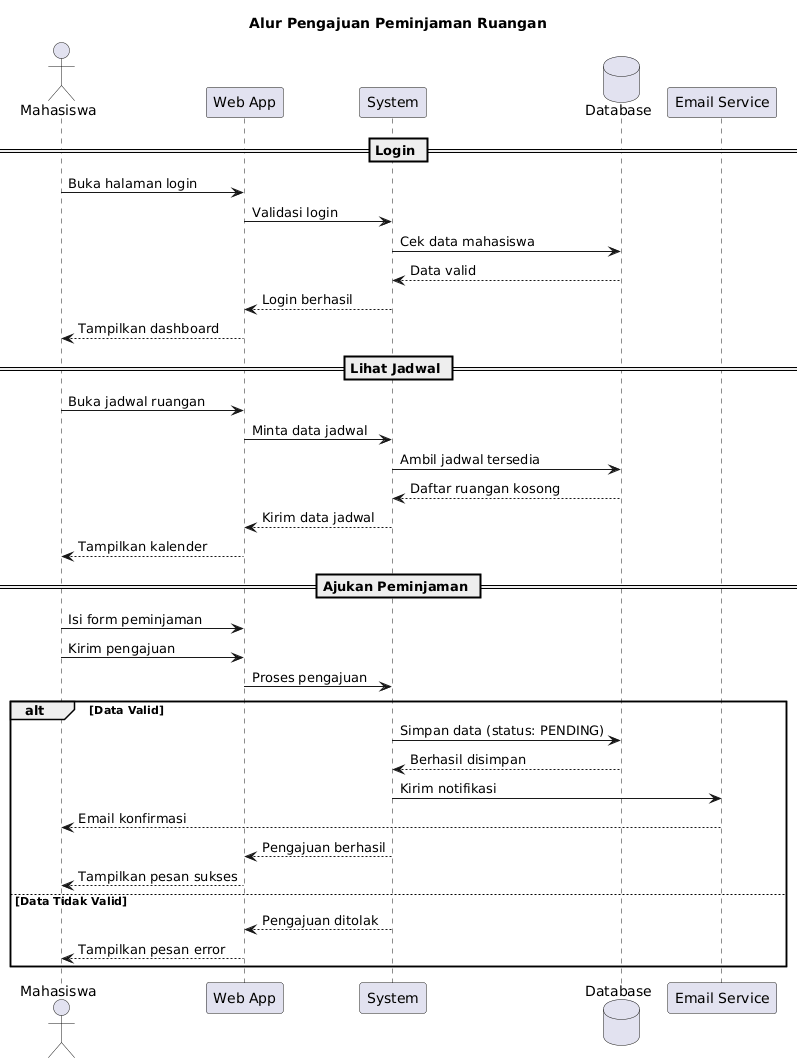
\includegraphics[width=0.8\textwidth]{gambar/media/image7.png}
    \caption{Sequence Diagram Pengajuan Peminjaman}
    \label{fig:sequence_pengajuan}
\end{figure}

Selanjutnya, mahasiswa membuka menu jadwal ruangan. Web App meminta data jadwal kepada System, yang kemudian mengambil data ketersediaan ruangan dari Database dan menampilkannya kembali kepada mahasiswa melalui Web App.

Mahasiswa kemudian mengisi dan mengirimkan formulir pengajuan peminjaman. System memvalidasi data pengajuan. Jika data valid, sistem menyimpan data peminjaman ke Database dengan status PENDING dan mengirimkan notifikasi email konfirmasi melalui Email Service. Web App menampilkan pesan bahwa pengajuan berhasil dikirim. Jika data tidak valid, sistem menolak pengajuan dan Web App menampilkan pesan kesalahan kepada mahasiswa.

Sequence diagram ini menunjukkan alur komunikasi antar komponen sistem secara berurutan dalam mendukung proses pengajuan peminjaman ruangan.

\subsubsection{Sequence Diagram Verifikasi Peminjaman}
Sequence diagram ini menggambarkan alur interaksi antara aktor Admin dengan Web App, System, Database, dan Email Service dalam proses verifikasi pengajuan peminjaman. Proses diawali ketika admin melakukan login melalui Web App. System memvalidasi kredensial admin dengan melakukan pengecekan ke Database. Jika login berhasil, sistem memberikan akses dan menampilkan dashboard admin.

Admin kemudian membuka daftar pengajuan peminjaman. Web App meminta data pengajuan dengan status PENDING kepada System, yang selanjutnya mengambil data tersebut dari Database dan menampilkannya dalam bentuk tabel. Admin memilih salah satu pengajuan untuk melihat detail lengkap, dan System mengambil serta menampilkan detail pengajuan dari Database.

Pada tahap pengambilan keputusan, admin dapat menyetujui atau menolak pengajuan. Jika pengajuan disetujui, System memperbarui status peminjaman menjadi APPROVED di Database dan mengirimkan notifikasi persetujuan kepada mahasiswa melalui Email Service. Jika pengajuan ditolak, System memperbarui status menjadi REJECTED beserta alasan penolakan dan mengirimkan notifikasi penolakan kepada mahasiswa. Setelah proses selesai, Web App menampilkan konfirmasi kepada admin.

\begin{figure}[htbp]
    \centering
    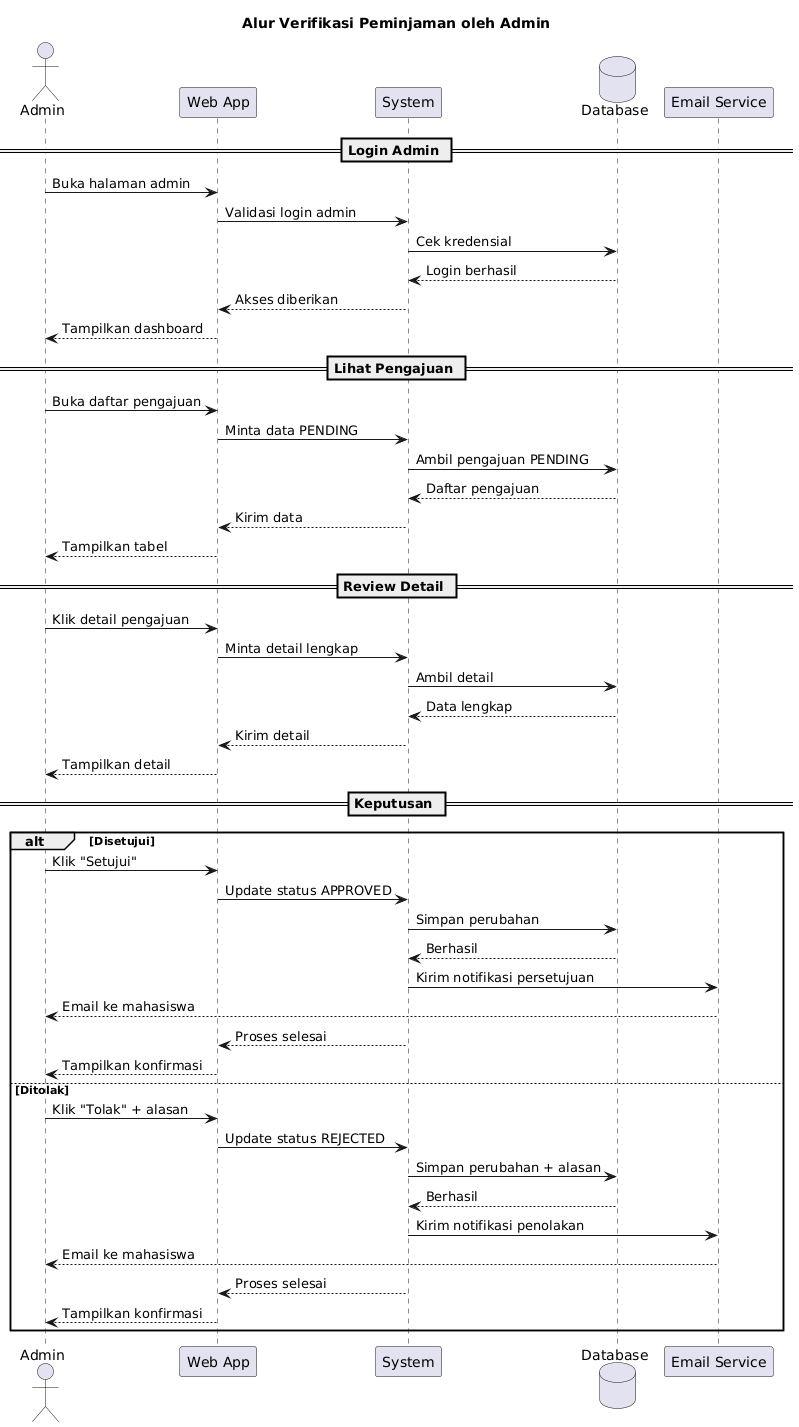
\includegraphics[width=0.8\textwidth]{gambar/media/image8.png}
    \caption{Sequence Diagram Verifikasi Peminjaman}
    \label{fig:sequence_verifikasi}
\end{figure}

Sequence diagram ini menunjukkan alur komunikasi sistem dalam memastikan setiap pengajuan peminjaman diverifikasi secara terkontrol dan terdokumentasi dengan baik.

\subsubsection{Sequence Diagram Verifikasi Kehadiran}
Sequence diagram ini menggambarkan alur interaksi antara aktor Security dengan Web App, System, dan Database dalam proses verifikasi kehadiran peminjam. Proses dimulai ketika security melakukan login melalui Web App, yang kemudian divalidasi oleh System dengan melakukan pengecekan kredensial ke Database. Setelah login berhasil, sistem menampilkan dashboard security.

\begin{figure}[htbp]
    \centering
    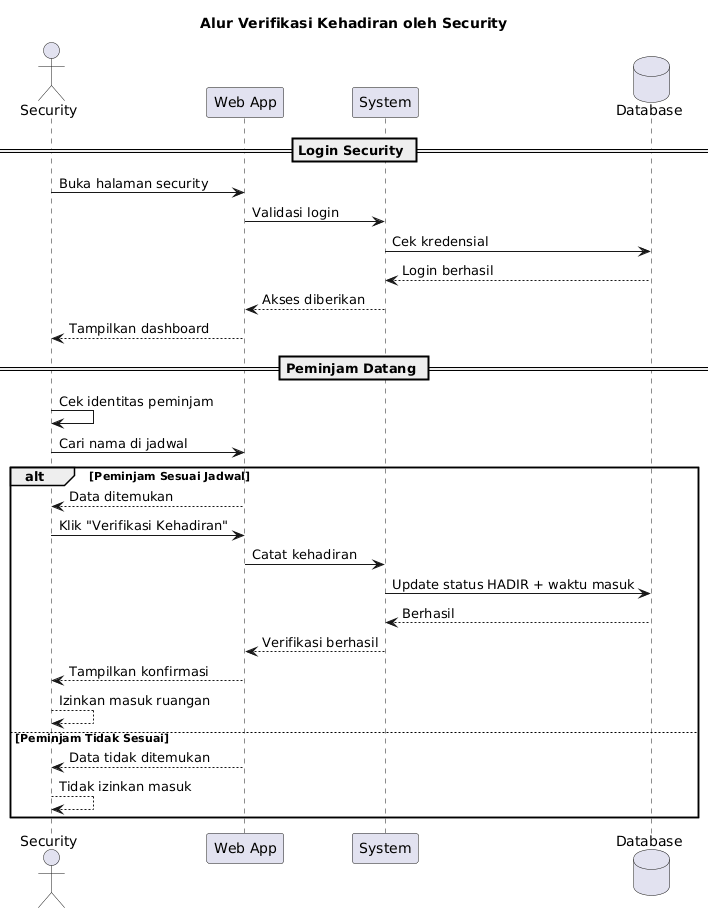
\includegraphics[width=0.8\textwidth]{gambar/media/image9.png}
    \caption{Sequence Diagram Verifikasi Kehadiran}
    \label{fig:sequence_kehadiran}
\end{figure}

Ketika peminjam datang, security melakukan pengecekan identitas dan mencari data peminjaman pada jadwal yang tersedia melalui Web App. System memproses permintaan tersebut dan memeriksa kesesuaian data dengan Database. Jika data peminjaman ditemukan dan sesuai jadwal, security melakukan verifikasi kehadiran. System kemudian mencatat kehadiran dengan memperbarui status menjadi HADIR beserta waktu masuk pada Database, dan menampilkan konfirmasi bahwa verifikasi berhasil sehingga peminjam diizinkan masuk ke ruangan.

Sebaliknya, apabila data peminjaman tidak ditemukan atau tidak sesuai, sistem menolak proses verifikasi dan security tidak memberikan izin masuk ke ruangan. Sequence diagram ini menunjukkan alur komunikasi sistem dalam memastikan bahwa hanya peminjam yang sah yang dapat menggunakan sarana dan prasarana kampus.

\subsection{Entity Relationship Diagram}

\begin{figure}[htbp]
    \centering
    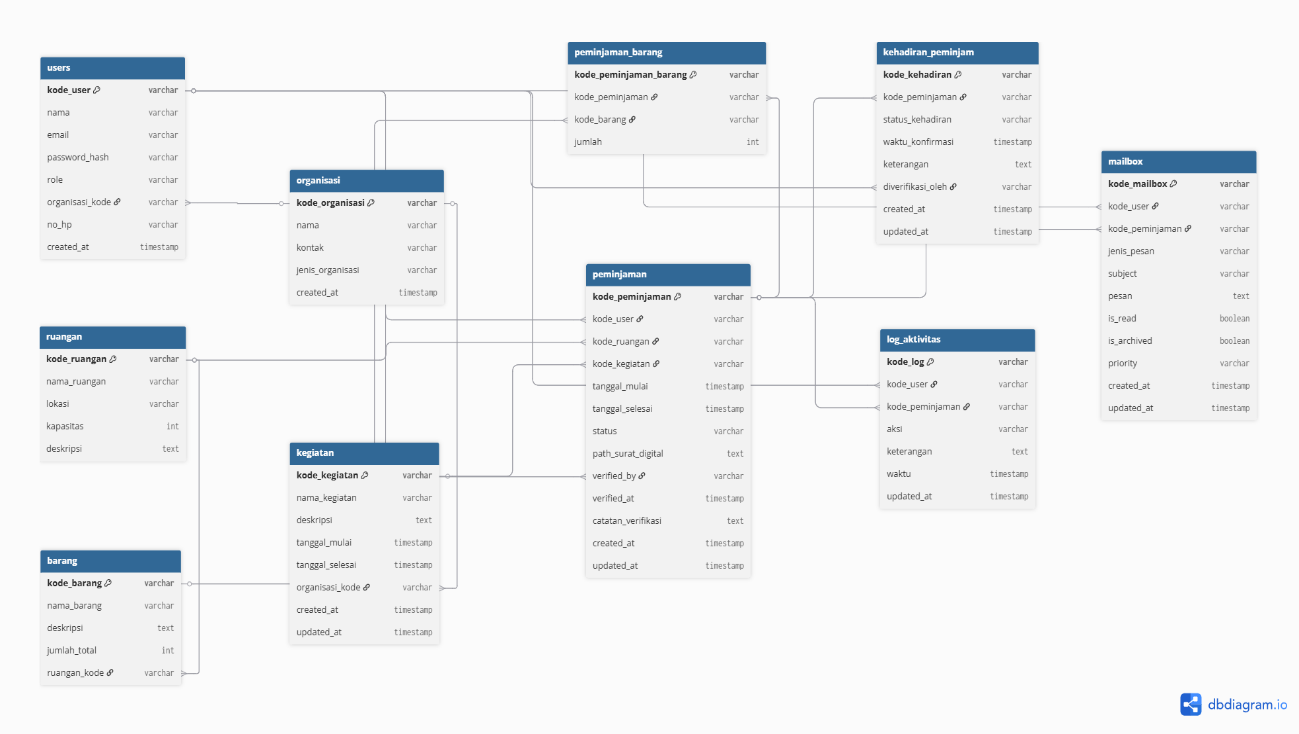
\includegraphics[width=0.8\textwidth]{gambar/media/image10.png}
    \caption{Entity Relationship Diagram}
    \label{fig:erd}
\end{figure}

Entity Relationship Diagram (ERD) digunakan untuk menggambarkan struktur basis data serta hubungan antar entitas yang terlibat dalam Sistem Informasi Peminjaman Sarana dan Prasarana Kampus. ERD ini menunjukkan keterkaitan antara data pengguna, data sarana dan prasarana, transaksi peminjaman, serta proses pendukung seperti verifikasi kehadiran, notifikasi, dan pencatatan aktivitas. Perancangan ERD dilakukan untuk memastikan integritas data dan mendukung pengolahan data menggunakan pendekatan Relational Database Management System (RDBMS).

\begin{table}[htbp]
    \centering
    \caption{Relasi Antar Entitas}
    \label{tab:relasi_entitas}
    \begin{tabular}{|c|l|l|l|p{6cm}|}
        \hline
        No. & Entitas Utama & Entitas Terkait & Jenis Relasi & Keterangan \\
        \hline
        1. & users & organisasi & One-to-Many & Satu organisasi dapat memiliki banyak pengguna \\
        \hline
        2. & users & peminjaman & One-to-Many & Satu pengguna dapat mengajukan lebih dari satu peminjaman \\
        \hline
        3. & ruangan & peminjaman & One-to-Many & Satu ruangan dapat digunakan dalam beberapa transaksi peminjaman \\
        \hline
        4. & kegiatan & peminjaman & One-to-Many & Satu kegiatan dapat menjadi dasar beberapa peminjaman \\
        \hline
        5. & peminjaman & peminjaman\_barang & One-to-Many & Satu peminjaman dapat memiliki lebih dari satu barang \\
        \hline
        6. & barang & peminjaman\_barang & One-to-One & Satu barang dapat tercatat pada banyak transaksi peminjaman \\
        \hline
        7. & peminjaman & kehadiran\_peminjam & One-to-Many & Setiap peminjaman memiliki satu data kehadiran \\
        \hline
        8. & users & mailbox & One-to-Many & Satu pengguna dapat menerima banyak notifikasi \\
        \hline
        9. & peminjaman & mailbox & One-to-Many & Satu peminjaman dapat menghasilkan banyak pesan \\
        \hline
        10. & users & log\_aktivitas & One-to-Many & Aktivitas pengguna tercatat dalam log sistem \\
        \hline
        11. & peminjaman & log\_aktivitas & One-to-Many & Aktivitas terkait peminjaman tercatat dalam log \\
        \hline
    \end{tabular}
\end{table}

Dengan perancangan ERD yang terstruktur dan relasi antar entitas yang jelas, Sistem Informasi Peminjaman Sarana dan Prasarana Kampus mampu mendukung pengelolaan data peminjaman secara terintegrasi dan konsisten. Struktur basis data ini menjadi acuan utama dalam implementasi sistem, khususnya dalam penerapan operasi CRUD serta pengelolaan data peminjaman, verifikasi, dan pelaporan pada tahap implementasi sistem.

\subsection{Class Diagram}
Class Diagram digunakan untuk menggambarkan struktur kelas dalam sistem beserta atribut, tipe data, serta hubungan antar kelas. Diagram ini merepresentasikan rancangan statis sistem yang menjadi dasar dalam proses implementasi, khususnya dalam pembuatan struktur database, model data, dan logika bisnis aplikasi.

\begin{table}[htbp]
    \centering
    \caption{Deskripsi Nama Kelas}
    \label{tab:deskripsi_kelas}
    \begin{tabular}{|c|l|p{9cm}|}
        \hline
        No. & Nama Kelas & Deskripsi \\
        \hline
        1. & Users & Merepresentasikan pengguna sistem dengan peran mahasiswa, sarpras, atau security \\
        \hline
        2. & Organisasi & Menyimpan data organisasi atau unit yang terkait dengan pengguna dan kegiatan \\
        \hline
        3. & Ruangan & Menyimpan data ruangan yang dapat dipinjam \\
        \hline
        4. & Barang & Menyimpan data barang atau inventaris yang dapat dipinjam \\
        \hline
        5. & Kegiatan & Menyimpan data kegiatan yang menjadi dasar peminjaman \\
        \hline
        6. & Peminjaman & Menyimpan data utama transaksi peminjaman sarana dan prasarana \\
        \hline
        7. & PeminjamanBarangDetail & Menyimpan detail barang yang dipinjam dalam satu transaksi \\
        \hline
        8. & KehadiranPeminjam & Menyimpan data verifikasi kehadiran peminjam \\
        \hline
        9. & Notifikasi & Menyimpan data notifikasi sistem kepada pengguna \\
        \hline
        10. & LogAktivitas & Menyimpan catatan aktivitas pengguna dalam sistem \\
        \hline
    \end{tabular}
\end{table}

\begin{figure}[htbp]
    \centering
    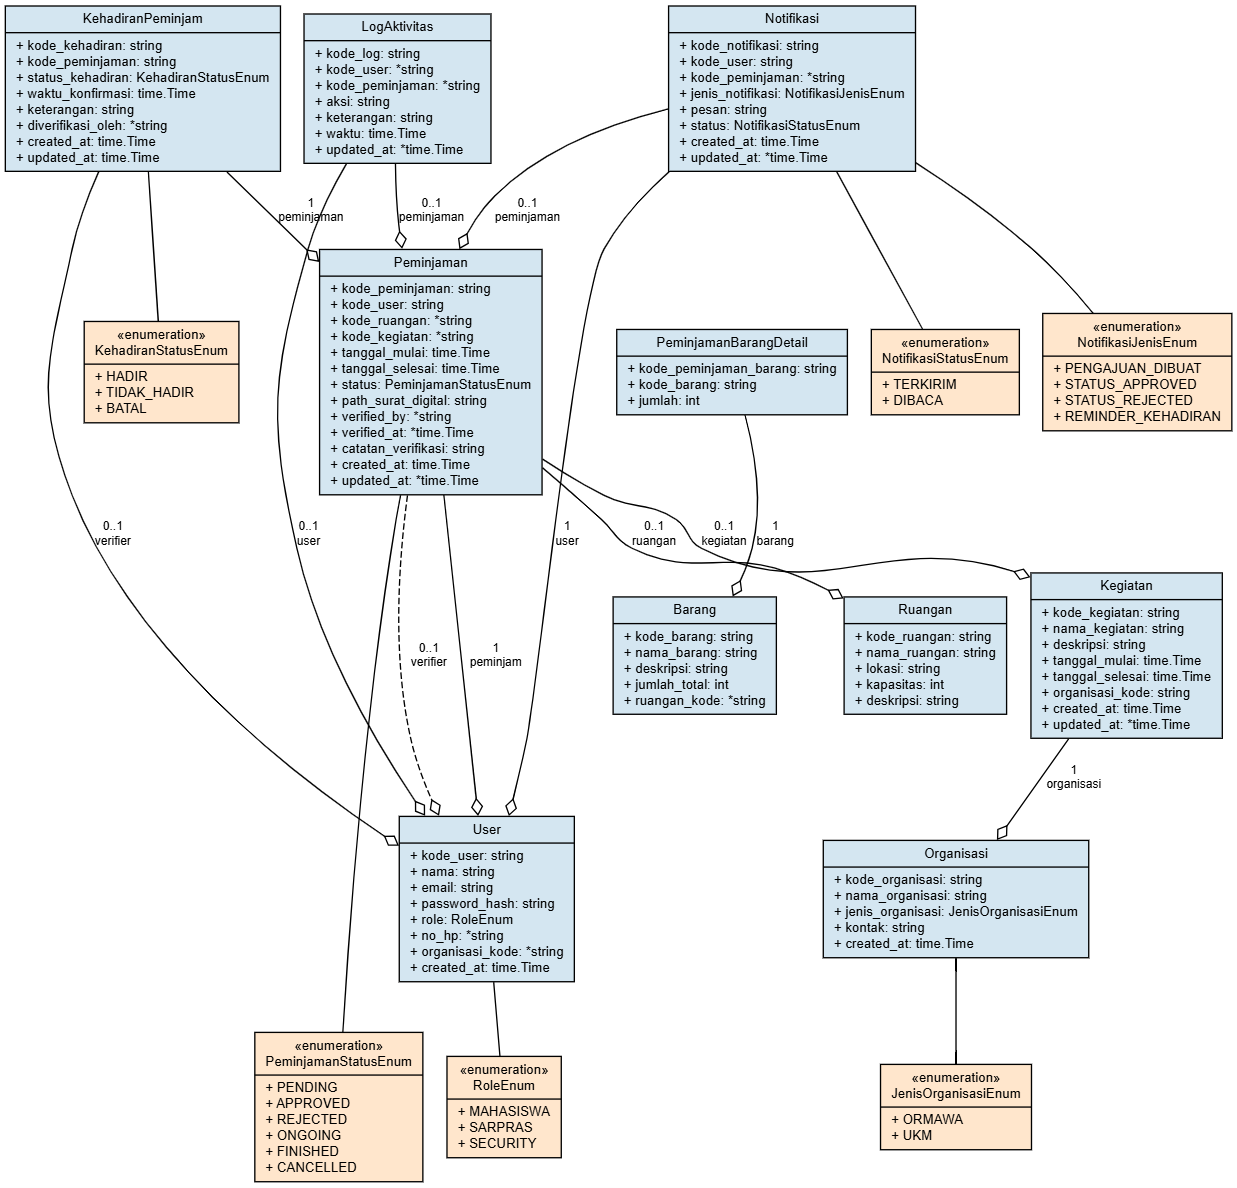
\includegraphics[width=0.8\textwidth]{gambar/media/image11.png}
    \caption{Class Diagram}
    \label{fig:class_diagram}
\end{figure}

Berdasarkan Class Diagram pada Gambar \ref{fig:class_diagram}, sistem peminjaman sarana dan prasarana kampus terdiri dari beberapa kelas utama, yaitu User, Peminjaman, Barang, Ruangan, Kegiatan, Organisasi, serta kelas pendukung seperti PeminjamanBarangDetail, KehadiranPeminjam, Notifikasi, dan LogAktivitas.
Kelas Peminjaman berperan sebagai pusat relasi yang menghubungkan pengguna dengan sarana dan prasarana yang dipinjam, kegiatan yang dilaksanakan, serta proses verifikasi dan kehadiran. Untuk menjaga konsistensi status dan peran dalam sistem, digunakan beberapa enumeration seperti RoleEnum, PeminjamanStatusEnum, KehadiranStatusEnum, NotifikasiJenisEnum, dan NotifikasiStatusEnum.

Dengan adanya Class Diagram ini, struktur kelas dan hubungan antar komponen dalam Sistem Informasi Peminjaman Sarana dan Prasarana Kampus dapat dipahami secara jelas. Class Diagram ini menjadi acuan dalam proses implementasi sistem, khususnya dalam pembuatan model data, pengelolaan relasi antar entitas, serta penerapan logika bisnis sesuai dengan kebutuhan sistem.

\subsection{BPMN Diagram}

\subsubsection{BPMN Proses Peminjaman}
BPMN Proses Peminjaman menggambarkan alur peminjaman sarana dan prasarana kampus secara \textit{end-to-end} yang melibatkan Mahasiswa, Sarpras, Security, dan Sistem Informasi. Proses dimulai dari login mahasiswa dan pengajuan peminjaman dengan melengkapi data serta unggah surat digital, kemudian sistem menyimpan pengajuan dan menetapkan status menunggu verifikasi.

\begin{figure}[htbp]
    \centering
    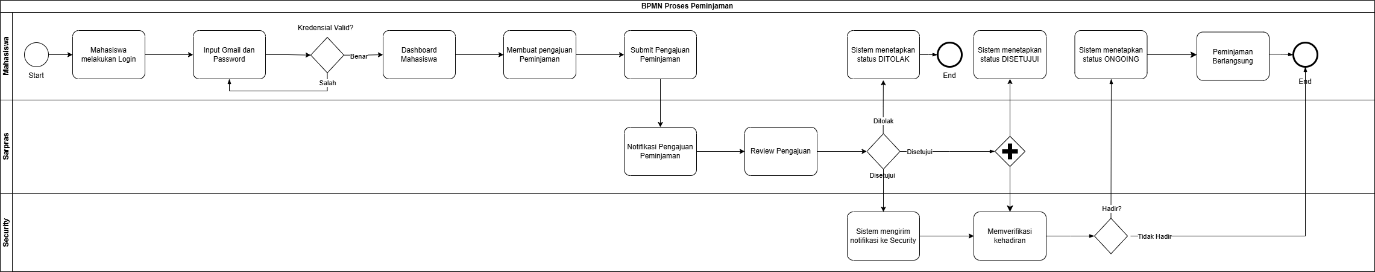
\includegraphics[width=0.8\textwidth]{gambar/media/image12.png}
    \caption{BPMN Proses Peminjaman}
    \label{fig:bpmn_peminjaman}
\end{figure}

Selanjutnya, Sarpras melakukan \textit{review} pengajuan untuk menentukan persetujuan atau penolakan, di mana pengajuan yang ditolak akan diakhiri oleh sistem dengan status DITOLAK, sedangkan pengajuan yang disetujui ditetapkan berstatus DISETUJUI dan diinformasikan kepada mahasiswa serta petugas keamanan. Pada hari pelaksanaan, Security melakukan verifikasi kehadiran peminjam; jika peminjam hadir, sistem memperbarui status peminjaman menjadi ONGOING yang menandakan kegiatan berlangsung, sedangkan jika peminjam tidak hadir, sistem mencatat kondisi tersebut dan proses peminjaman dinyatakan selesai.

\subsubsection{BPMN Verifikasi Peminjaman}
BPMN Verifikasi Peminjaman menggambarkan alur pemeriksaan dan pengambilan keputusan terhadap pengajuan peminjaman sarana dan prasarana oleh pihak Sarpras. Proses dimulai ketika pengajuan peminjaman masuk ke dalam sistem, kemudian Sarpras melakukan login dan mengakses dashboard untuk meninjau serta memeriksa kelengkapan dan kebenaran data pengajuan, seperti identitas peminjam, jenis sarana atau prasarana, jadwal penggunaan, dan dokumen pendukung.

\begin{figure}[htbp]
    \centering
    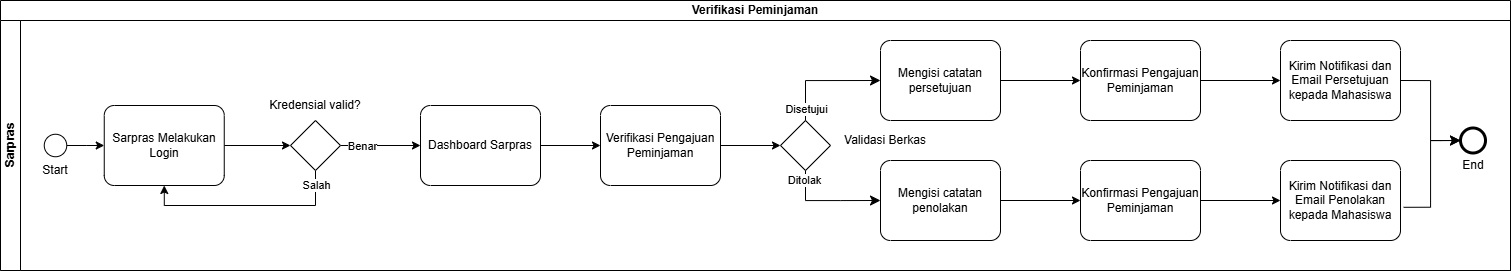
\includegraphics[width=0.8\textwidth]{gambar/media/image13.png}
    \caption{BPMN Verifikasi Peminjaman}
    \label{fig:bpmn_verifikasi}
\end{figure}

Berdasarkan hasil verifikasi tersebut, Sarpras mengambil keputusan untuk menyetujui atau menolak pengajuan peminjaman. Pada kondisi pengajuan disetujui, Sarpras mengisi catatan persetujuan, kemudian sistem mengonfirmasi pengajuan dan secara otomatis mengirimkan notifikasi serta email persetujuan kepada mahasiswa. Sebaliknya, apabila pengajuan ditolak, Sarpras mengisi alasan penolakan yang dicatat oleh sistem, kemudian sistem mengonfirmasi penolakan dan mengirimkan notifikasi serta email penolakan kepada mahasiswa. Proses verifikasi peminjaman dinyatakan selesai setelah keputusan akhir disampaikan kepada pemohon dan tercatat dalam sistem.

\subsubsection{BPMN Verifikasi Kehadiran}
BPMN Verifikasi Kehadiran Peminjam menggambarkan proses pemeriksaan kehadiran peminjam sarana dan prasarana kampus yang dilakukan oleh petugas Security pada hari pelaksanaan peminjaman. Proses dimulai ketika Security melakukan login ke sistem dan mengakses dashboard untuk melakukan verifikasi kehadiran peminjam berdasarkan data peminjaman yang telah disetujui.

\begin{figure}[htbp]
    \centering
    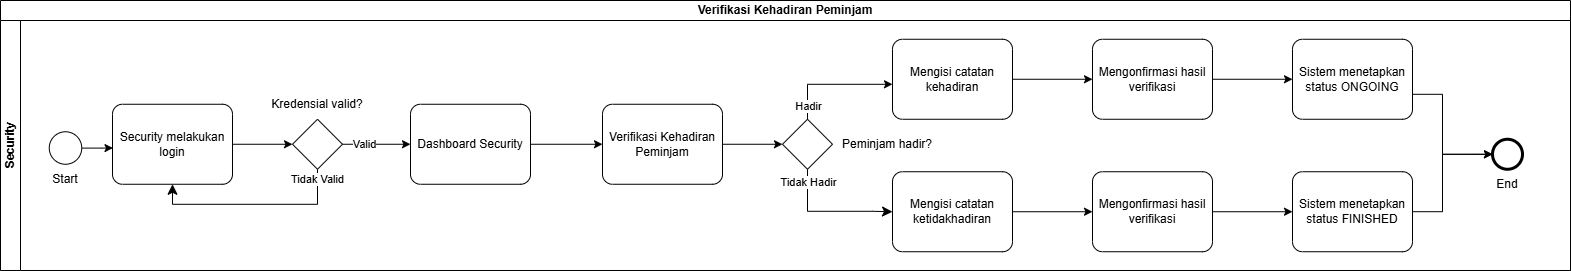
\includegraphics[width=0.8\textwidth]{gambar/media/image14.png}
    \caption{BPMN Verifikasi Kehadiran}
    \label{fig:bpmn_kehadiran}
\end{figure}

Selanjutnya, Security melakukan pemeriksaan apakah peminjam hadir sesuai dengan jadwal yang ditentukan, di mana pada kondisi peminjam hadir Security mengisi catatan kehadiran dan sistem mengonfirmasi hasil verifikasi dengan menetapkan status peminjaman menjadi ONGOING, sedangkan pada kondisi peminjam tidak hadir Security mengisi catatan ketidakhadiran dan sistem mengonfirmasi hasil verifikasi dengan menetapkan status peminjaman menjadi FINISHED. Proses verifikasi kehadiran ini berfungsi sebagai kontrol akhir untuk memastikan bahwa penggunaan sarana dan prasarana kampus berjalan sesuai dengan persetujuan dan ketentuan yang berlaku.

\subsection{Lingkungan Implementasi Sistem}
(Isi bab 4 akan dilengkapi nanti)

\subsection{Kesimpulan}
(Isi bab 5 akan dilengkapi nanti)


% References
\printbibliography[heading=bibintoc, title={DAFTAR PUSTAKA}]

% Lampiran
% \clearpage
\phantomsection
\addcontentsline{toc}{chapter}{LAMPIRAN}
\chapter*{LAMPIRAN}

% Reset figure numbering for appendix
\setcounter{figure}{0}
\renewcommand{\thefigure}{L.\arabic{figure}}
\renewcommand{\figurename}{Gambar}
\renewcommand{\cftfigpresnum}{Gambar }
\setlength{\cftfignumwidth}{4.5em}

\section*{Lampiran A: Hasil Pengujian \textit{Code Coverage Backend}}

Lampiran ini menyajikan hasil pengujian \textit{code coverage} \textit{backend} menggunakan \textit{testing framework} Go. Hasil ditampilkan dalam bentuk laporan HTML yang menunjukkan persentase \textit{coverage} dan detail kode yang telah diuji (\textit{covered}) maupun belum diuji (\textit{not covered}).

\subsection*{A.1 Ringkasan \textit{Code Coverage}}

Ringkasan hasil pengujian menunjukkan total \textit{code coverage} sebesar 31,9\%. Modul inti (\textit{auth\_service}, \textit{code\_generator}, \textit{kehadiran\_service}, \textit{peminjaman\_service}) telah mencapai tingkat keterujian tinggi.

\begin{figure}[H]
    \centering
    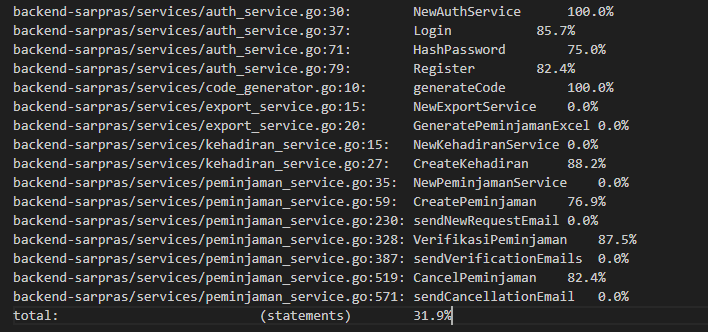
\includegraphics[width=0.9\textwidth]{gambar/media/image25.png}
    \caption{Ringkasan \textit{Code Coverage Backend}}
    \label{fig:coverage_summary}
\end{figure}

\subsection*{A.2 Detail \textit{Coverage}: \textit{Auth Service}}

Detail \textit{coverage} \textit{Auth Service} menunjukkan sebagian besar kode telah tercakup pengujian (hijau), termasuk fungsi kritis seperti \textit{login} dan \textit{register}.

\begin{figure}[H]
    \centering
    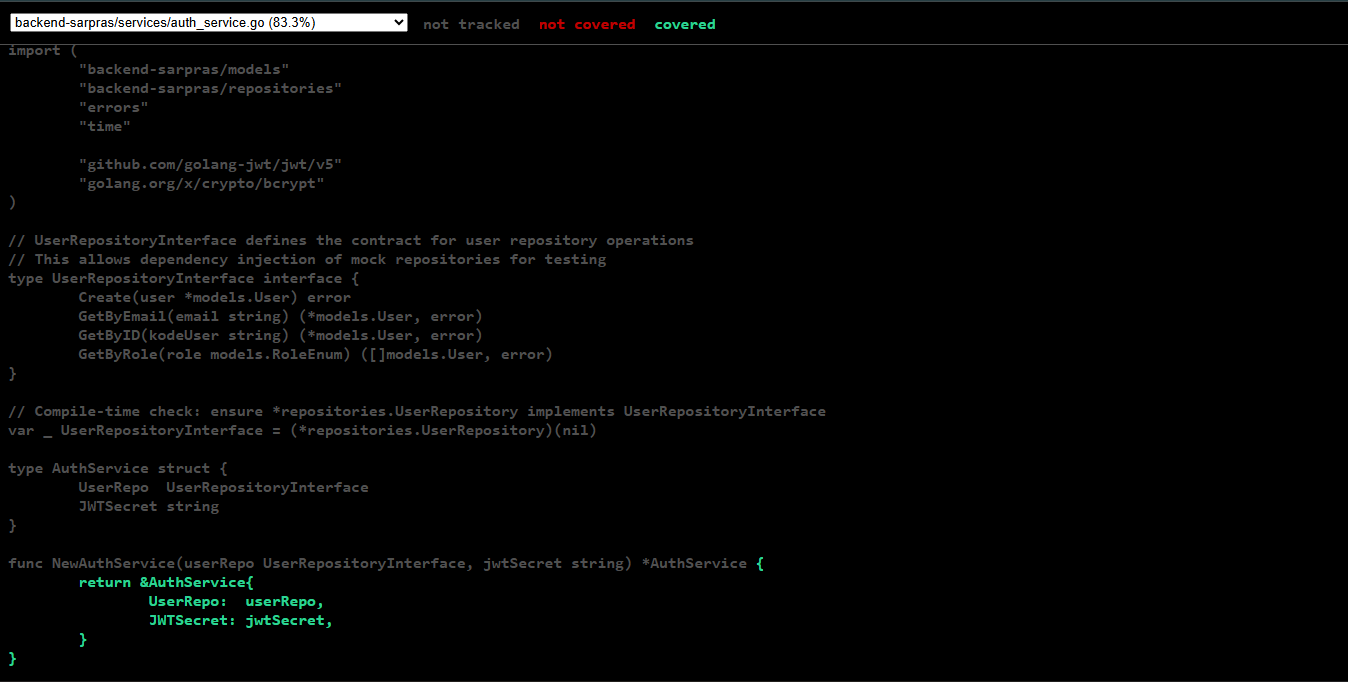
\includegraphics[width=0.9\textwidth]{gambar/media/auth service.png}
    \caption{Detail \textit{Coverage} \textit{Auth Service}}
    \label{fig:coverage_auth}
\end{figure}

\subsection*{A.3 Detail \textit{Coverage}: \textit{Kehadiran Service}}

Detail \textit{coverage} \textit{Kehadiran Service} menunjukkan tingkat \textit{coverage} tinggi (88,2\%), dengan fungsi utama \texttt{CreateKehadiran} telah diuji menyeluruh.

\begin{figure}[H]
    \centering
    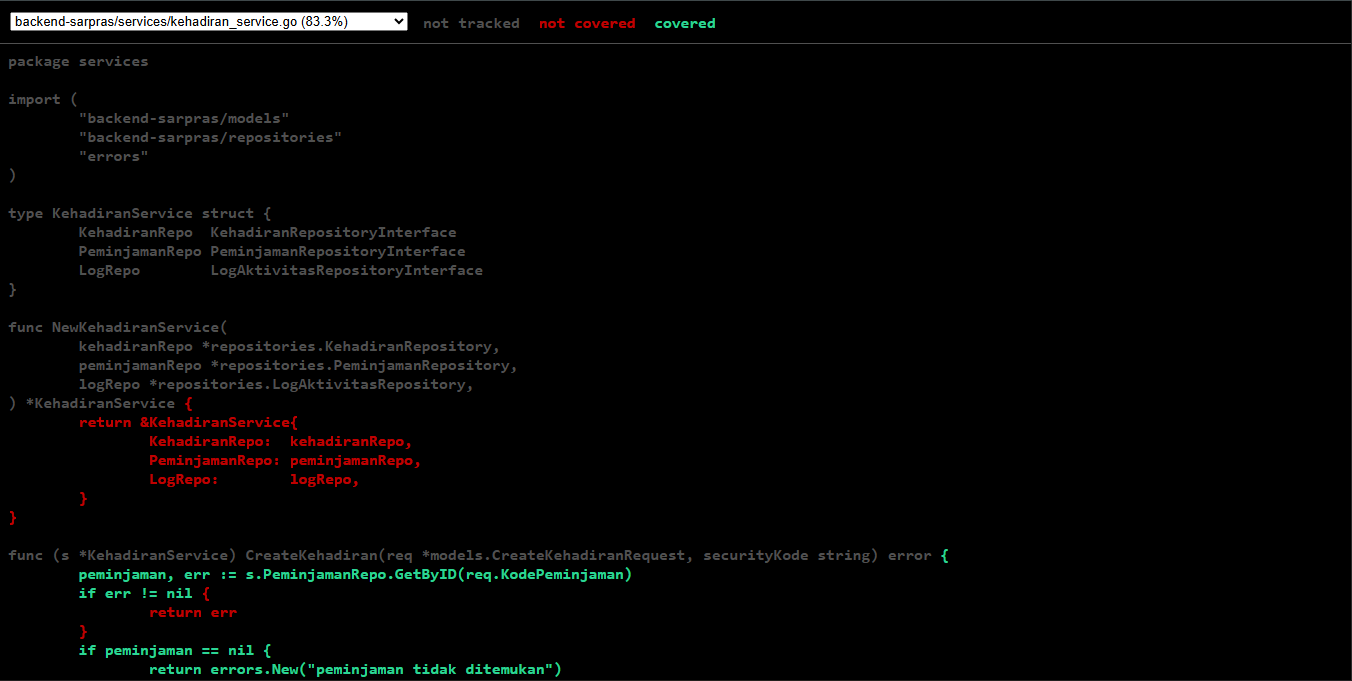
\includegraphics[width=0.9\textwidth]{gambar/media/kehadiran service.png}
    \caption{Detail \textit{Coverage} \textit{Kehadiran Service}}
    \label{fig:coverage_kehadiran}
\end{figure}

\subsection*{A.4 Detail \textit{Coverage}: \textit{Peminjaman Service}}

Detail \textit{coverage} \textit{Peminjaman Service} menunjukkan tingkat \textit{coverage} baik untuk fungsi inti (pengajuan, verifikasi, pembatalan peminjaman).

\begin{figure}[H]
    \centering
    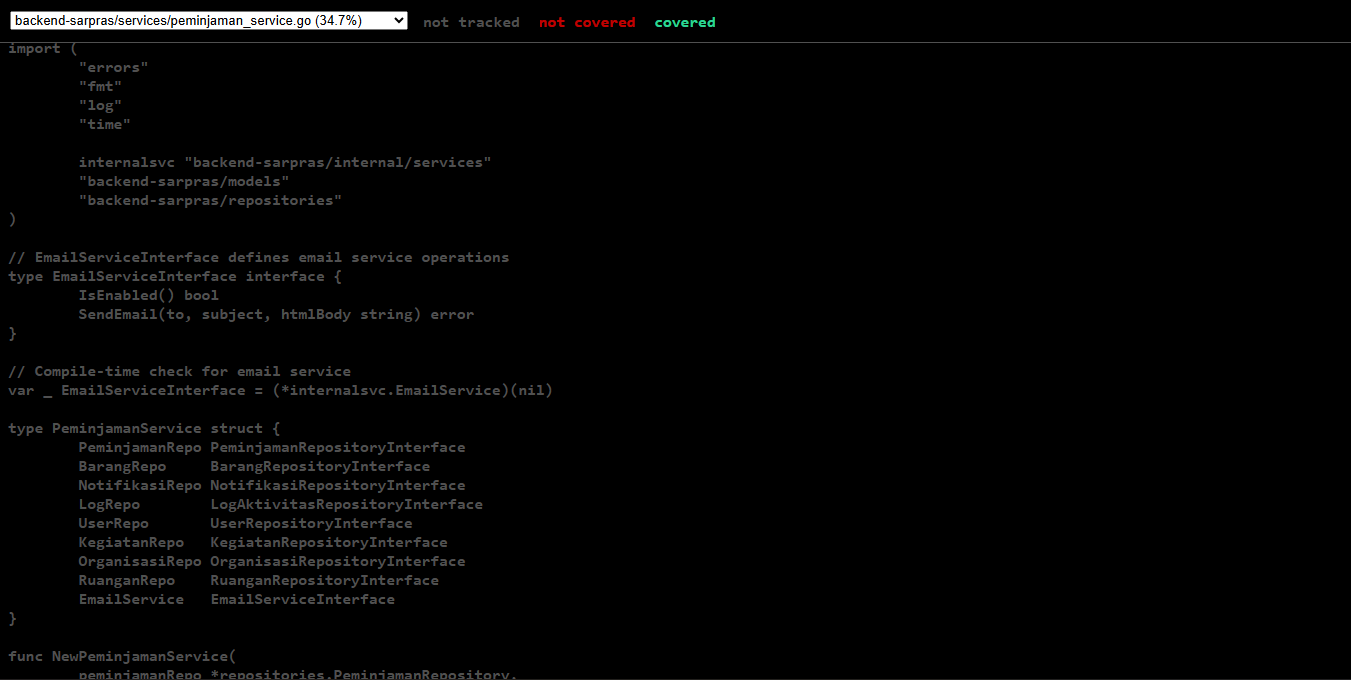
\includegraphics[width=0.9\textwidth]{gambar/media/peminjaman service.png}
    \caption{Detail \textit{Coverage} \textit{Peminjaman Service}}
    \label{fig:coverage_peminjaman}
\end{figure}

\section*{Lampiran B: Dokumentasi Wawancara}

Dokumentasi wawancara dengan staf Sarana dan Prasarana sebagai bagian proses pengumpulan data dan analisis kebutuhan sistem.

\begin{figure}[H]
    \centering
    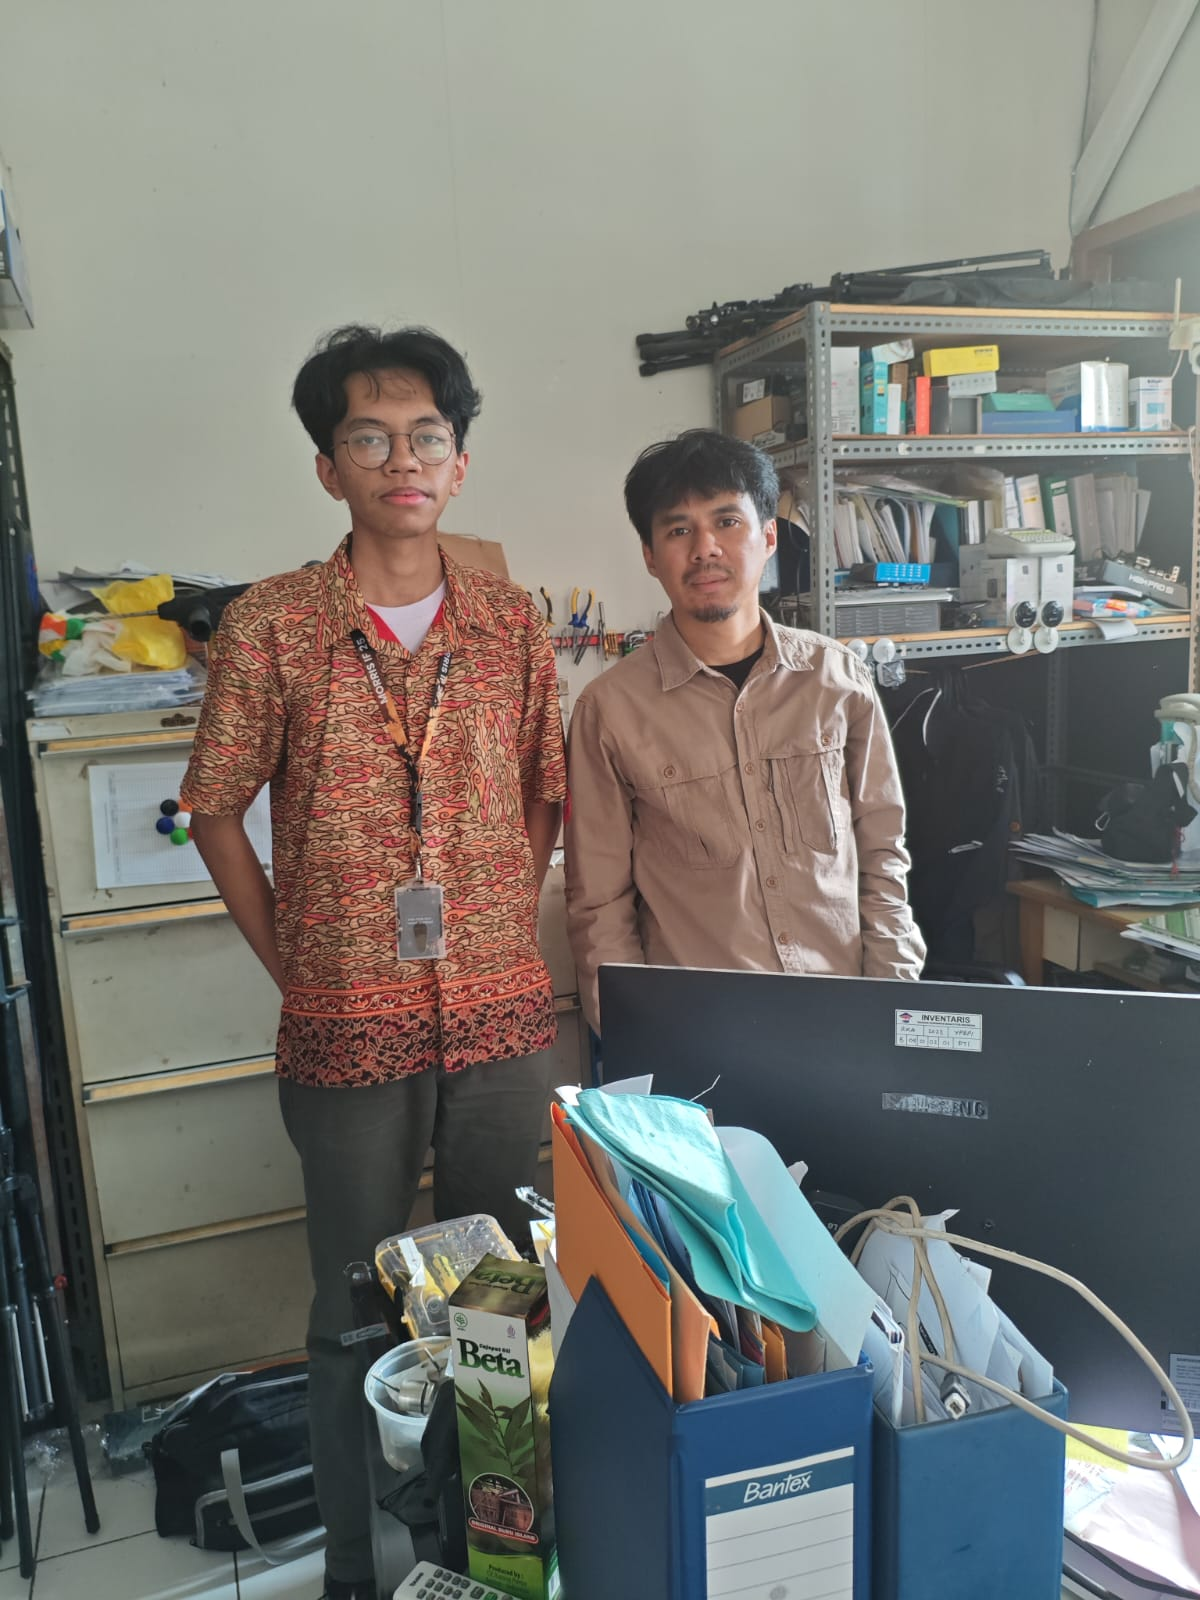
\includegraphics[width=0.5\textwidth]{gambar/media/coblong.jpeg}
    \caption{Dokumentasi Wawancara dengan Staf Sarana dan Prasarana}
    \label{fig:dokumentasi_wawancara}
\end{figure}


\end{document}
